\chapter{Introduction}
\label{sec:Introduction}


Gyeli is a Bantu A80 language spoken in southern Cameroon and northern Equatorial Guinea.  
The Gyeli speakers, who are called \textit{Bagyeli}, are hunter-gatherers constituting the western-most ``Pygmy'' group in Central Africa. Their forest foraging lifestyle  distinguishes them from agriculturalist Bantu groups in the area, opposing ``Bagyeli'' and ``Bantu'' ethnically, although linguistically, they are all Bantu speakers.

This chapter provides extra-linguistic and methodological context to the grammatical description. The introduction contains four parts. I will provide a general discussion of Gyeli's language situation including information on the name, linguistic classification, speaker numbers, language contact, and dialects. I will pay special attention to the village \textit{Ngolo}, on whose speakers I base this description.  In the second part, I introduce the Gyeli speakers, the environment they live in, and give a rough outline of their culture and subsistence. I will then address various aspects of the methodology I used in compiling the grammatical description of Gyeli. This includes information on the data, but also information on what I consider the ``speech community'' that provided data for the linguistic description. I conclude the chapter with a user guide to this grammar by providing a content overview of each chapter and a summary of basic grammatical features that frequently occur in glossed example sentences to make them easily accessible to the reader. 

The introduction also highlights two distinctive features of this grammar.  First, the grammatical description is based on a multimodal language documentation corpus compiled within the ``Bagyeli/Bakola'' {\itshape DoBeS} (Documentation of Endangered Languages) project.  This corpus includes an extensive amount of natural texts of diverse genres as well as approximately 170 hours of elicitations, developed over the course of 4 years, 19 months of which were spent in the field. Following the ``Boasian trilogy'' \citep{evans2006}, the Gyeli grammar includes a grammatical description, a collection of annotated texts, and a small dictionary. In contrast to Boas, however, my text corpus does not only contain narratives, but also other text genres that reflect language use in everyday face-to-face communication.  While the grammar is largely based on actual language use, elicitations supplement the range of constructions I was able to uncover. As such, this grammar is the product of an effort to synthesize language description and language documentation traditions. With advances in technology and archiving, not only are text and elicitation data available in a transcribed print version, but the primary video and audio data are available in the {\itshape The Language Archive} \citep{grimm2020a}, ensuring accountability and reproducibility of my claims.

In order to ``let the language speak for itself'', this grammar is organized according to the form-to-function principle, rather than by semantic categories. \chapref{sec:TAM} on the verbal complex, for instance, is structured according to predicate types rather than by functional domains, such as tense, aspect, mood, and negation. In order  to facilitate finding functional categories, e.g.\ for typologists, I provide a summary of functional categories and their location in the grammar in the introduction of the chapter. Similarly, I summarize the semantic category of numerals at the end of \chapref{sec:NP}.


 


\section{The Gyeli language}
\label{sec:Gyeli}

The Gyeli language situation is characterized by a relatively small number of  speakers scattered in a vast area that is shared with a multitude of other languages and ethnic groups.
Estimations of the population of Gyeli speakers range from 2,200, following \citet[27]{renaud76}, to around 5,000 as proposed by \citet[215]{ngima2001}. In the \textit{Ethnologue}, \citet{lewis09} gives figures of 4,250 Gyeli speakers in Cameroon and 29 in Equatorial Guinea. Based on a sociolinguistic survey conducted with my colleague Emmanuel Ngue Um in 2010,  we estimate 4,000 to 5,000 speakers.\footnote{The difficulty in establishing a more precise estimate arises for various reasons. Gyeli speakers often live in remote villages and settlements which are not easily accessible. They often do not possess identity cards, so that they are not officially registered with the authorities. Another difficulty in estimating population numbers is due to mobility patterns. Gyeli speakers, though becoming more sedentary in terms of permanent villages, are highly mobile and regularly switch villages. Therefore, it is hard to say how many people exactly live in a village.}

The region in which Gyeli is spoken measures about 12,500km\textsuperscript{2} (which corresponds to about 4,800mi\textsuperscript{2}). Unlike many other languages in the world, especially in the Indo-European context with its national languages, Gyeli is neither the only (or predominant) language in the region nor restricted to one contiguous geographic area. Instead, Gyeli is one out of nine languages in the area as shown below in Map \ref{Fig:Gyeli-map}.  Naturally, there is intensive language contact between the languages of the region. Gyeli speakers are shifting to the languages of their farmer neighbors, a trend which both fragments Gyeli into different dialects and contributes to the language's endangerment.  I will discuss each of these aspects in turn in more detail below.


\subsection{The language's name}
\label{sec:name}

Gyeli is known under a variety of names, sometimes depending on who is talking about the language. In the \textit{Ethnologue}, for instance, \citet{lewis09} calls the language \textit{Gyele} with the code ISO 639-3: gyi. It also lists the following alternate names that are also used to designate the same language (however, not specifying who uses which name): Babinga, Bagiele, Bagyele, Bajele, Bajeli, Bako, Bakola, Bakuele, Bekoe, Bogyel, Bogyeli, Bondjiel, Giele, Gieli, Gyeli, Likoya.

There are two patterns observable within the various names. First, some names have a prefix of the general form \textit{Ba}- and some are prefixless.
The \textit{Ba}- prefix, or the corresponding prefixes \textit{Bo}- and \textit{Be}- used in other languages, are typical Bantu prefixes of the plural noun class 2 of the human gender designating groups of people. Thus, the language names with a prefix derive from a group of people rather than their language. 

Although this might be unusual for the anglophone Bantu tradition, I refer to the speaker group as {\itshape Bagyeli}, using the {\itshape Ba}- prefix instead of the bare stem. The reason for this is that the Gyeli speakers and their neighboring Bantu groups use this term (rather than {\itshape Gyeli}), both in local languages and in French. In contrast, most ethnic groups of the area, for instance the Kwasio, Mabi, Bulu, and Yasa, do not receive  the {\itshape Ba}- prefix. Since the prefix is then not used consistently for all ethnic groups, it seems that it is really part of the name for Gyeli speakers. When talking about the language, however, I use the bare stem {\itshape Gyeli}.\footnote{In contrast to the \textit{Ethnologue}, I use the spelling of Gyeli with an {\textlangle}i{\textrangle} in the end instead of Gyele with an {\textlangle}e{\textrangle} at the end since my language consultants prefer this variant.}

Another pattern, apart from a name with or without a prefix, is the similarities of forms to either ``Gyeli'' or ``Kola''. There are variants such as -{\itshape jele}, -{\itshape giele}, -{\itshape jeli}, -{\itshape gyel} or {\itshape Gieli} which can be subsumed under variants of ``Gyeli''. Other variants such as -{\itshape kola}, -{\itshape ko} or -{\itshape koya} can be subsumed under variants of ``Kola''. %\footnote{Babinga and Koya are very widespread and general Bantu names for forest foragers in Central Africa. What are they derived from (in Proto-Bantu)?} 
These two different names correlate with geographic areas. 
Speakers in the northern part of the Gyeli language zone call their language {\itshape Kola}, speakers in the central and southern part call it {\itshape Gyeli}, but it is nevertheless considered the same language. Accordingly, the speakers are called {\itshape Bagyeli} in the center and south, and {\itshape Bakola} in the north. Since the speech community on which I base this grammar is located in the southern-central part of the Gyeli/Kola language zone (see Map \ref{Fig:Gyeli-map}), I use the name {\itshape Gyeli} rather than {\itshape Kola}.

{\itshape Bagyeli} and {\itshape Bakola} are terms used both as endonym (the way a group calls itself) and exonym (the name used for a group by outsiders).\footnote{Groups such as the Mabi and Ngumba, both dialects of Kwasio, as well as the Bulu, seem to use these terms. Exonyms used by other groups such as the Yasa or Bakoko, as represented in Map \ref{Fig:Gyeli-map}, require further investigation since I was not in direct contact with them during my fieldwork. \citet[29-30]{renaud76} discusses exonyms as used by the Basaa, Bulu, Fang, Mabi, and Ngumba. They are all related to the terms ``Gyeli'' and ``Kola''.} There is, however, an alternate exonym used by all local Bantu neighbors, namely the French word \textit{pygmées} ``Pygmies''. It seems to be a convenient cover term for short-sized hunter-gatherers in Central Africa, especially since people not familiar with the ethnic and linguistic situation in Central Africa usually associate more with the term ``Pygmy'' than with ``Bagyeli'' or ``Bakola''. I will, however, not use this term for several reasons. First, the term ``Pygmy'' generally has a pejorative connotation (although this is certainly not always implied by the Bantu farmer neighbors who use it). Second, it implies a certain homogeneity among such Central African forest foragers which is, in all reality, not existent. So-called ``Pygmy'' groups differ considerably in terms of language, type of contact with their farming neighbors, settlement patterns, and hunting techniques, just to mention a few differences.

\largerpage
\subsection{Classification}
With about 2000 languages out of the about 7000 languages world-wide, the African continent is linguistically very rich and diverse. For Cameroon alone, the \textit{Ethnologue} lists 278 living languages. \figref{Fig:Gyeli-Africa} shows the geographic location of the Gyeli language within Africa.

\begin{figure}
% \includegraphics[width=8.5cm]{figures/Gyeli-in-Africa.png}
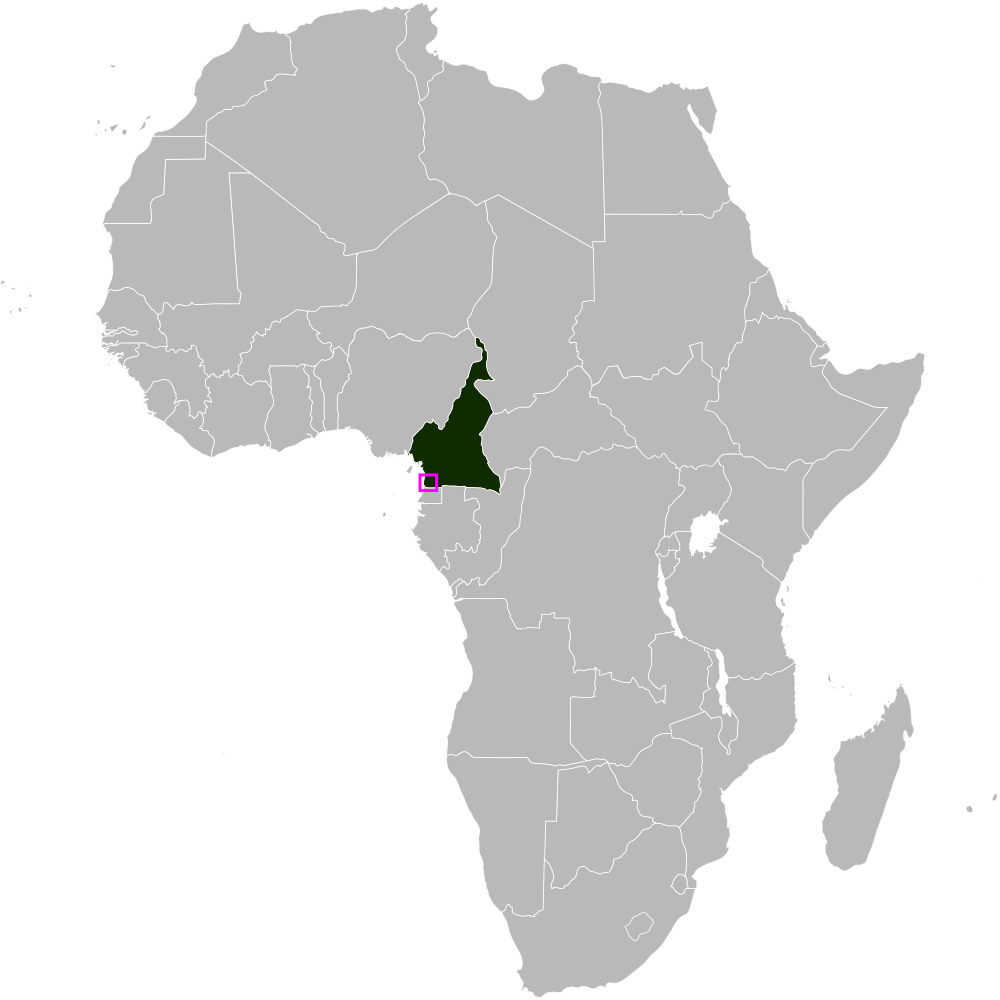
\includegraphics[height=.4\textheight]{figures/cameroon.pdf}
%\includegraphics[width=\textwidth]{Gyeli-in-Africa.png}
\caption{Location of Gyeli and Cameroon in Africa\\{\tiny based on \url{https://commons.wikimedia.org/wiki/File:Locator_map_of_Cameroon_in_Africa.svg} CC-BY-SA Shosholoza }}
\label{Fig:Gyeli-Africa}
\end{figure}




\subsubsection*{Classification within Niger-Congo} Languages of Cameroon mostly belong to the Niger-Congo languages, as does Gyeli. With roughly 1,500 languages, Niger-Congo constitutes the biggest language family in Africa, as classified by, for instance, \citet{williamson2000}. \figref{Fig:ClassBantu} visualizes the classification of Gyeli within the Niger-Congo family. The figure is a simplified adaptation from \citet{williamson2000} and \citet{lewis09}. Within Niger-Congo, Gyeli belongs to the narrow Bantu languages and, within Bantu, to the Makaa-Njem group (A80). 



\begin{figure}
\resizebox{9cm}{!}{
\begin{forest}  forked edges
[Niger-Congo
    [{\dots}]
    [Atlantic-Congo
        [{\dots}]
        [Benue-Congo
            [{\dots}]
            [Southern Bantoid
                [{\dots}]
                [Narrow Bantu
                    [{\dots}]
                    [Makaa-Njem Group (A80)
                        [{\dots}]
                        [\textbf{Gyeli (A801)}]
                    ]
                ]
            ]
        ]
    ]
]
\end{forest}
}
%   \setlength {\unitlength}{1mm}
% \begin {picture}(70,60)
% \put (-20,60){\textbf{Niger-Congo}}
% \put (-10,50){$\bullet$ Atlantic-Congo}
% \put (0,40){$\bullet$ Benue-Congo}
% \put (10,30){$\bullet$ Southern Bantoid}
% \put (20,20){$\bullet$ Narrow Bantu}
% \put (30,10){$\bullet$ Makaa-Njem Group (A80)}
% \put (40,0){$\bullet$ \textbf{Gyeli (A801)}}
% \end {picture}
\caption {The classification of Gyeli within the Niger-Congo family, based on \citet{williamson2000} and \citet{lewis09}}
\label {Fig:ClassBantu}
\end {figure}


\subsubsection*{Classification within Bantu} With about 500 members, the Bantu languages form the biggest subfamily of the Niger-Congo languages and, at the same time, cover a vast territory stretching from the borders of Nigeria and Cameroon all the way to east and south Africa. Probably the most famous member of the Bantu languages is Swahili, a language spoken in Tanzania, Kenya and in parts of other surrounding countries such as Mozambique, Uganda, Burundi, the Democratic Republic of the Congo, and Somalia. Even though Swahili is spoken thousands of kilometers away, many linguistic similarities to the Bantu languages in Cameroon can still be observed.

\citet{guthrie71} classifies the Bantu languages areal-typologically. As a referential classification, his model is, with slight modifications, still the most widely accepted one, although the classification is based on geography, and not on linguis\-tic-genetic criteria%
, as \citet[46]{maho2001} points out. %%overfull line
% \citep[46]{maho2001}.
Guthrie divides the Bantu-speaking area into fifteen zones and names each zone with a capital letter (A, B, C, D, E, F, G, H, K, L, M, N, P, R, S), as explained in \citet[3]{nurse03} and shown in \figref{Fig:Bantu-zones}. The J zone represented in the map is a later addition by the {\itshape Tervuren} team, which groups parts of Guthrie's zones D and E together.\footnote{Letters I, O, or Q were never used for zone designations.} As \citet[337]{philippson2019} explain, there is also a widespread convention to refer to later revisions in the classification of some Bantu languages by double letters, e.g. Rundi JD62, where the second letter refers to the zone that the language was previously grouped with.
Each zone is further subdivided into smaller parts which are labeled by decimals. For instance, the Bantu zone A is divided into the subzones A10, A20, A30, A40, A50, A60, A70, A80, and A90.
\begin{figure}

% 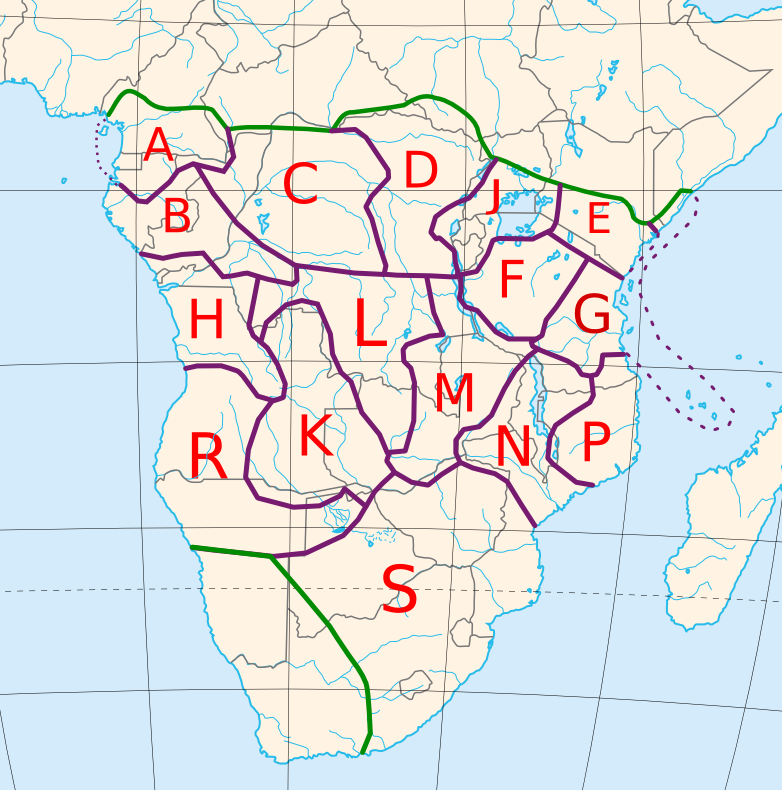
\includegraphics[width=8.5cm]{figures/Bantuzones.png}
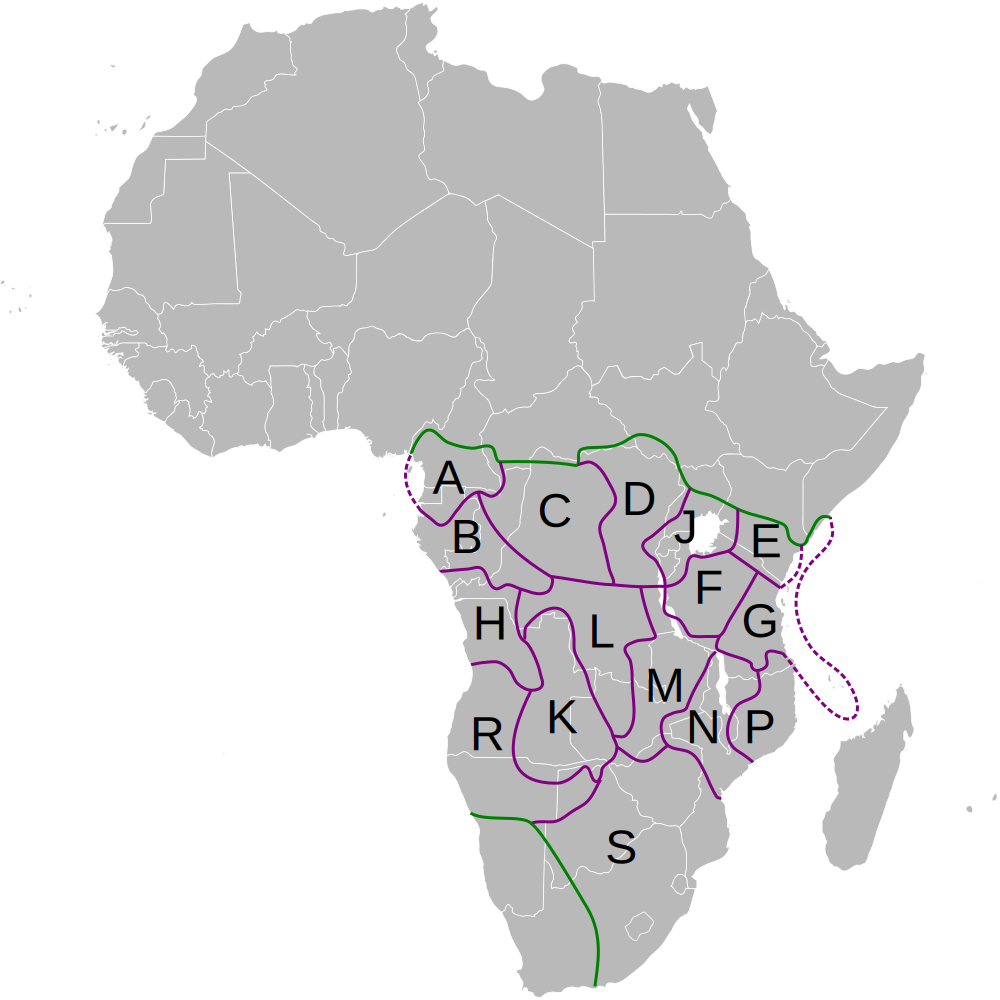
\includegraphics[width=8.5cm]{figures/bantuzones.pdf}
\caption{Guthrie's Bantu zones (with Tervuren's J zone)\\{\tiny based on \url{https://commons.wikimedia.org/wiki/File:Locator_map_of_Cameroon_in_Africa.svg} CC-BY-SA Shosholoza }}
\label{Fig:Bantu-zones}
\end{figure}



Bantuists often distinguish between northwestern Bantu languages, also called ``Forest'' languages, and non-northwestern languages, referred to as ``Savannah'' languages. Northwestern Bantu includes Guthrie's zones A and B at its core and, to a lesser extent, also (parts of) zones C, D, and H, depending on the author \citep[10]{nurse08}. Gyeli, as a Bantu A language, is a northwestern Bantu language. \citet[5]{nurse03} state that northwestern Bantu languages ``form exceptions to many possible generalizations for Bantu'' and show lots of ``non-Bantu'' features. This is also true for Gyeli which is, for instance, a much more isolating language than its Savannah relatives.


\subsubsection*{Classification within the Makaa-Njem group (A80)}
The languages of each subzone are specified by adding further digits to the subzone code. For instance, Gyeli as part of the subzone A80, also called the Makaa-Njem group, is referenced by A801. The internal classification of A80 according to the Guthrie code\footnote{I follow \posscitet{maho2009} updates of the codes, which include the additions of some coding features to Guthrie's system. Dialects are marked by a letter following the digits. A lower-case letter is used in Guthrie's original classification, an upper-case letter for newly added dialects.} is shown in \tabref{Tab:A80}.  The table is sorted by the Guthrie code as updated by \citet{maho2009}. The second column lists the ISO code, if existing, as used in the {\itshape Ethnologue}, followed by the glottocode used by the {\itshape Glottolog}. The fourth column gives the name and possibly alternate names used for the language.\footnote{A valuable discussion of the geographic distribution of Bantu A80 languages, including maps, is given in \citet{cheucle2014}.}


\begin{table}

\begin{tabularx}{\textwidth}{lllX}
\lsptoprule
Guthrie code & ISO code & Glottocode &  Name(s) \\ 
 \midrule
{\bfseries A801} & {\bfseries gyi} & {\bfseries gyel1242} & {\bfseries Gyele, Bagyeli, Bakola} \\
A802 & ukh & ukhw1241 & Ukwadjo, Ukhwejo \\
A803 &      & shiw1234 & Shiwa, Shiwe, Oshieba, Ossyeba\\
A81 &  nmg  & kwas1243 &  Mvumbo, Kwasio, Ngumba, Magbea\\
A82 & sox & soca1235 & So \\
A83 & mcp & maka1304 &  Makaa, South Makaa \\
A83A &   & bebe1249 &  Bebend \\
A83B &    & mbwa1238 & Mbwaanz \\
A83C &    & seku1238 & Shikunda, Sekunda \\
A831 & mkk & byep1241 & Byep, North Makaa \\
A832 & biw & kolc1235 & Bekol, Kol, Bikele  \\
A84 & njy  &  njye1238 & Njem, Nyem, Zimu \\
A841 &   &  & Bajue, Badwee \\
A842 & ozm  & koon1245 & Koonzime, Nzime \\
A85a &      & kuna1267 & Nkonabeeb, Konabem \\
A85b & bkw & bekw1242 & Bekwel, Bakwele \\
A86a &  &  menz1238 & Mezime, Medjime \\
A86b & mgg & mpon1254 &  Mpompon, Mpongmpong, Bombo \\
A86c  & mcx & mpie1238 & Mpiemo, Mbimu \\
A87  & bmw &  bomw1238 & Bomwali, Sanghasangha \\
\lspbottomrule
\end{tabularx}
\caption{Languages of the Makaa-Njem group (A80)}
\label{Tab:A80}
\end{table}

Gyeli receives the Guthrie code A801 by \citet{maho2001} and the ISO code 639-3: gyi.   The  three-digit Guthrie code indicates that the language was not represented in the original classification, but added later by Maho, since a third digit is added to the code if the language's affiliation is not clear or it is closely related to several other languages of the group  \citep[46]{maho2001}.

One reason for Gyeli's unclear status may be more ethnic or historical than reflecting a synchronic linguistic reality. The Bagyeli have a special status in that they are not ethnically Bantu. They are forest foragers who have lived in symbiosis with sedentary Bantu farmer communities over a long period of time. \citet[154]{ruhlen94} expresses a widely held view: ``It is assumed that Pygmies once spoke their own language(s), but that, through living in symbiosis with other Africans, in prehistorical times, they adopted languages belonging to these two families [Niger-Kordofanian and Nilo-Saharan].''\footnote{While the term ``Niger-Kordofanian'' was used by authors such as \citet{ruhlen94} and \citet{welmers73}, the current literature predominantly refers to this language family  as ``Niger-Congo.''}
As with many other examples in the history of language classification, ethnic affiliation and/or historic assumptions may have influenced linguistic classification. In the Gyeli case, this may have lead to confusion as to how to integrate a hunter-gatherer language (with a supposedly distinctive linguistic history) into a farmer language group since the other languages of the Makaa-Njem group are all spoken by farming communities. In synchronic linguistic description, however, neither the ethnic background of the speakers nor an unknown linguistic history should play a role in classifying a language.

Another reason for Gyeli's unclear status within the A80 group in \posscitet{maho2009} classification may be due to the problematic differentiation between ``language'' and ``dialect''. The Gyeli language is indeed closely related to Kwasio (A81). As previous literature by \citet{renaud76} suggests, Gyeli is so similar to Kwasio that \citet{bahuchet2006} considers it a dialect of the latter. This view may, however, be biased since Renaud bases his description on a Gyeli variety that is closest to Kwasio. There are other Gyeli varieties which are less similar to Kwasio, but instead more influenced by other neighboring farmer languages as I will explain in \sectref{sec:LangCon} and \sectref{sec:dialects} on language contact and dialects of Gyeli. 

Just like the \textit{Ethnologue} and \citet{maho2009}, I consider Gyeli to be a language of its own, containing several dialects. Whether Gyeli is a language or a dialect (of Kwasio) is not entirely uncontroversial, for indeed, the Bagyeli in close vicinity to Kribi and along the road between Kribi and Lolodorf are in close contact with Kwasio speakers and their variety is very similar to Kwasio. There are, however, two main reasons why I treat Gyeli as a language of its own. First, there are still significant differences in linguistic features. For instance, the Gyeli tense system is highly reduced segmentally in comparison to the farmer languages of the area. While all related and neighboring Bantu farmer languages use inflectional morphemes to express tense, tense-mood in Gyeli is only marked by tonal contrasts.
 Second, mutual intelligibility between Kwasio and Gyeli is limited. All Bagyeli speak, or at least understand, Kwasio for socio-economic reasons since they have learned the language of higher prestige in a multilingual setting.  My Kwasio language assistants state, however, that when the Bagyeli speak their own ``real'' or ``deep'' language, i.e.\ when they do not make efforts to be understood by their farming neighbors, Kwasio speakers do not understand them.



\subsection{Language contact}
\label{sec:LangCon}
% There are several farmer languages Gyeli borrows from and even shifts to while the Gyeli language is fragmented into several varieties which are also in contact with one another. Figure *** gives a visual representation of the language contact situation including the various actors as well as directions of borrowing. The plain arrows symbolize orientation towards a language of higher prestige while the dotted arrows stand for the direction borrowings take from one language/variety into another. 

%[GYELI'S LANGUAGE CONTACT SITUATION {\AND} BORROWING DIRECTIONS]

%\noindent The three different layers represent different levels of prestige. French as the language of the former colonizors and still language of (higher) education enjoys the highest prestige in this scenario. On a mid level are several Bantu farmer languages Gyeli is in contact with and that, at the same time, are also partially in contact with one another. These farmer languages still have a higher prestige than Gyeli because the Bantu farmers have a better education and more political power in comparison to the marginalized and mostly illiterate Bagyeli. On the lowest prestige level is Gyeli with several varieties. Depending on which farmer language a Gyeli group is mainly in contact with different dialects have emerged. Just like the farmer languages, also the various Gyeli dialects are in contact with one another and spread borrowings between different dialects. In the following, I will look at each of the actor groups in turn, starting with inter-ethnic contact between the Bagyeli and Bantu farmers.

The Gyeli language is part of a highly complex language contact situation. There are several groups and several directions of borrowing  which altogether make for an intricate language contact scenario. The Gyeli speakers are in contact with eight Bantu farmer languages which, in turn, are influenced by the colonial language French. 

\figref{Fig:Gyeli-map} provides a map of the Gyeli speaking area and its contact languages.\footnote{\figref{Fig:Gyeli-map} is based on the United Nations map No. 4227 (2004). Thanks to Sebastian Nordhoff for reworking an earlier version of this map.} Gyeli, marked by the dotted area, is roughly spoken from the river Nyong in the north into Equatorial Guinea just across the river Ntem in the south. To the west, the area is delimited by the Atlantic Ocean while it stretches almost to Ebolowa in the east. Bantu farmer contact languages are represented by capital letters in different colors. The colors correspond to different language subgroups within the Bantu A group, as listed in \tabref{Tab:Contact} below. For instance, the languages in green, Batanga and Yasa, are part of the A30 group. Contact languages of Gyeli varieties studied within the DoBeS project (\sectref{sec:Dobes}) receive additional graphical marking by a shaded area.  Basaa is marked by a yellow shade, Bulu by red, and the two areas in different hues of blue, Mabi and Ngumba, are dialects of Kwasio.

The variety I describe in this grammar is based on data from {\itshape Ngolo} village in the Bulu region. It is located about one to two kilometers to the southeast of the Bulu village {\itshape Nko'olong}. Officially, Ngolo, the Gyeli variant for the Bulu name Nko'olong, belongs to the Bulu village.  Comparative data from both Gyeli villages in other language contact areas and neighboring Bantu languages have been collected within the DoBeS language documentation project. Gyeli villages are marked with boxes around the village names such as Ngolo, Lebdjom, Bibira, and Namikoumbi. Nziou in the Mabi area and Nko'olong in the Bulu area are locations of comparative data collection in neighboring Bantu languages.

\begin{figure}
% 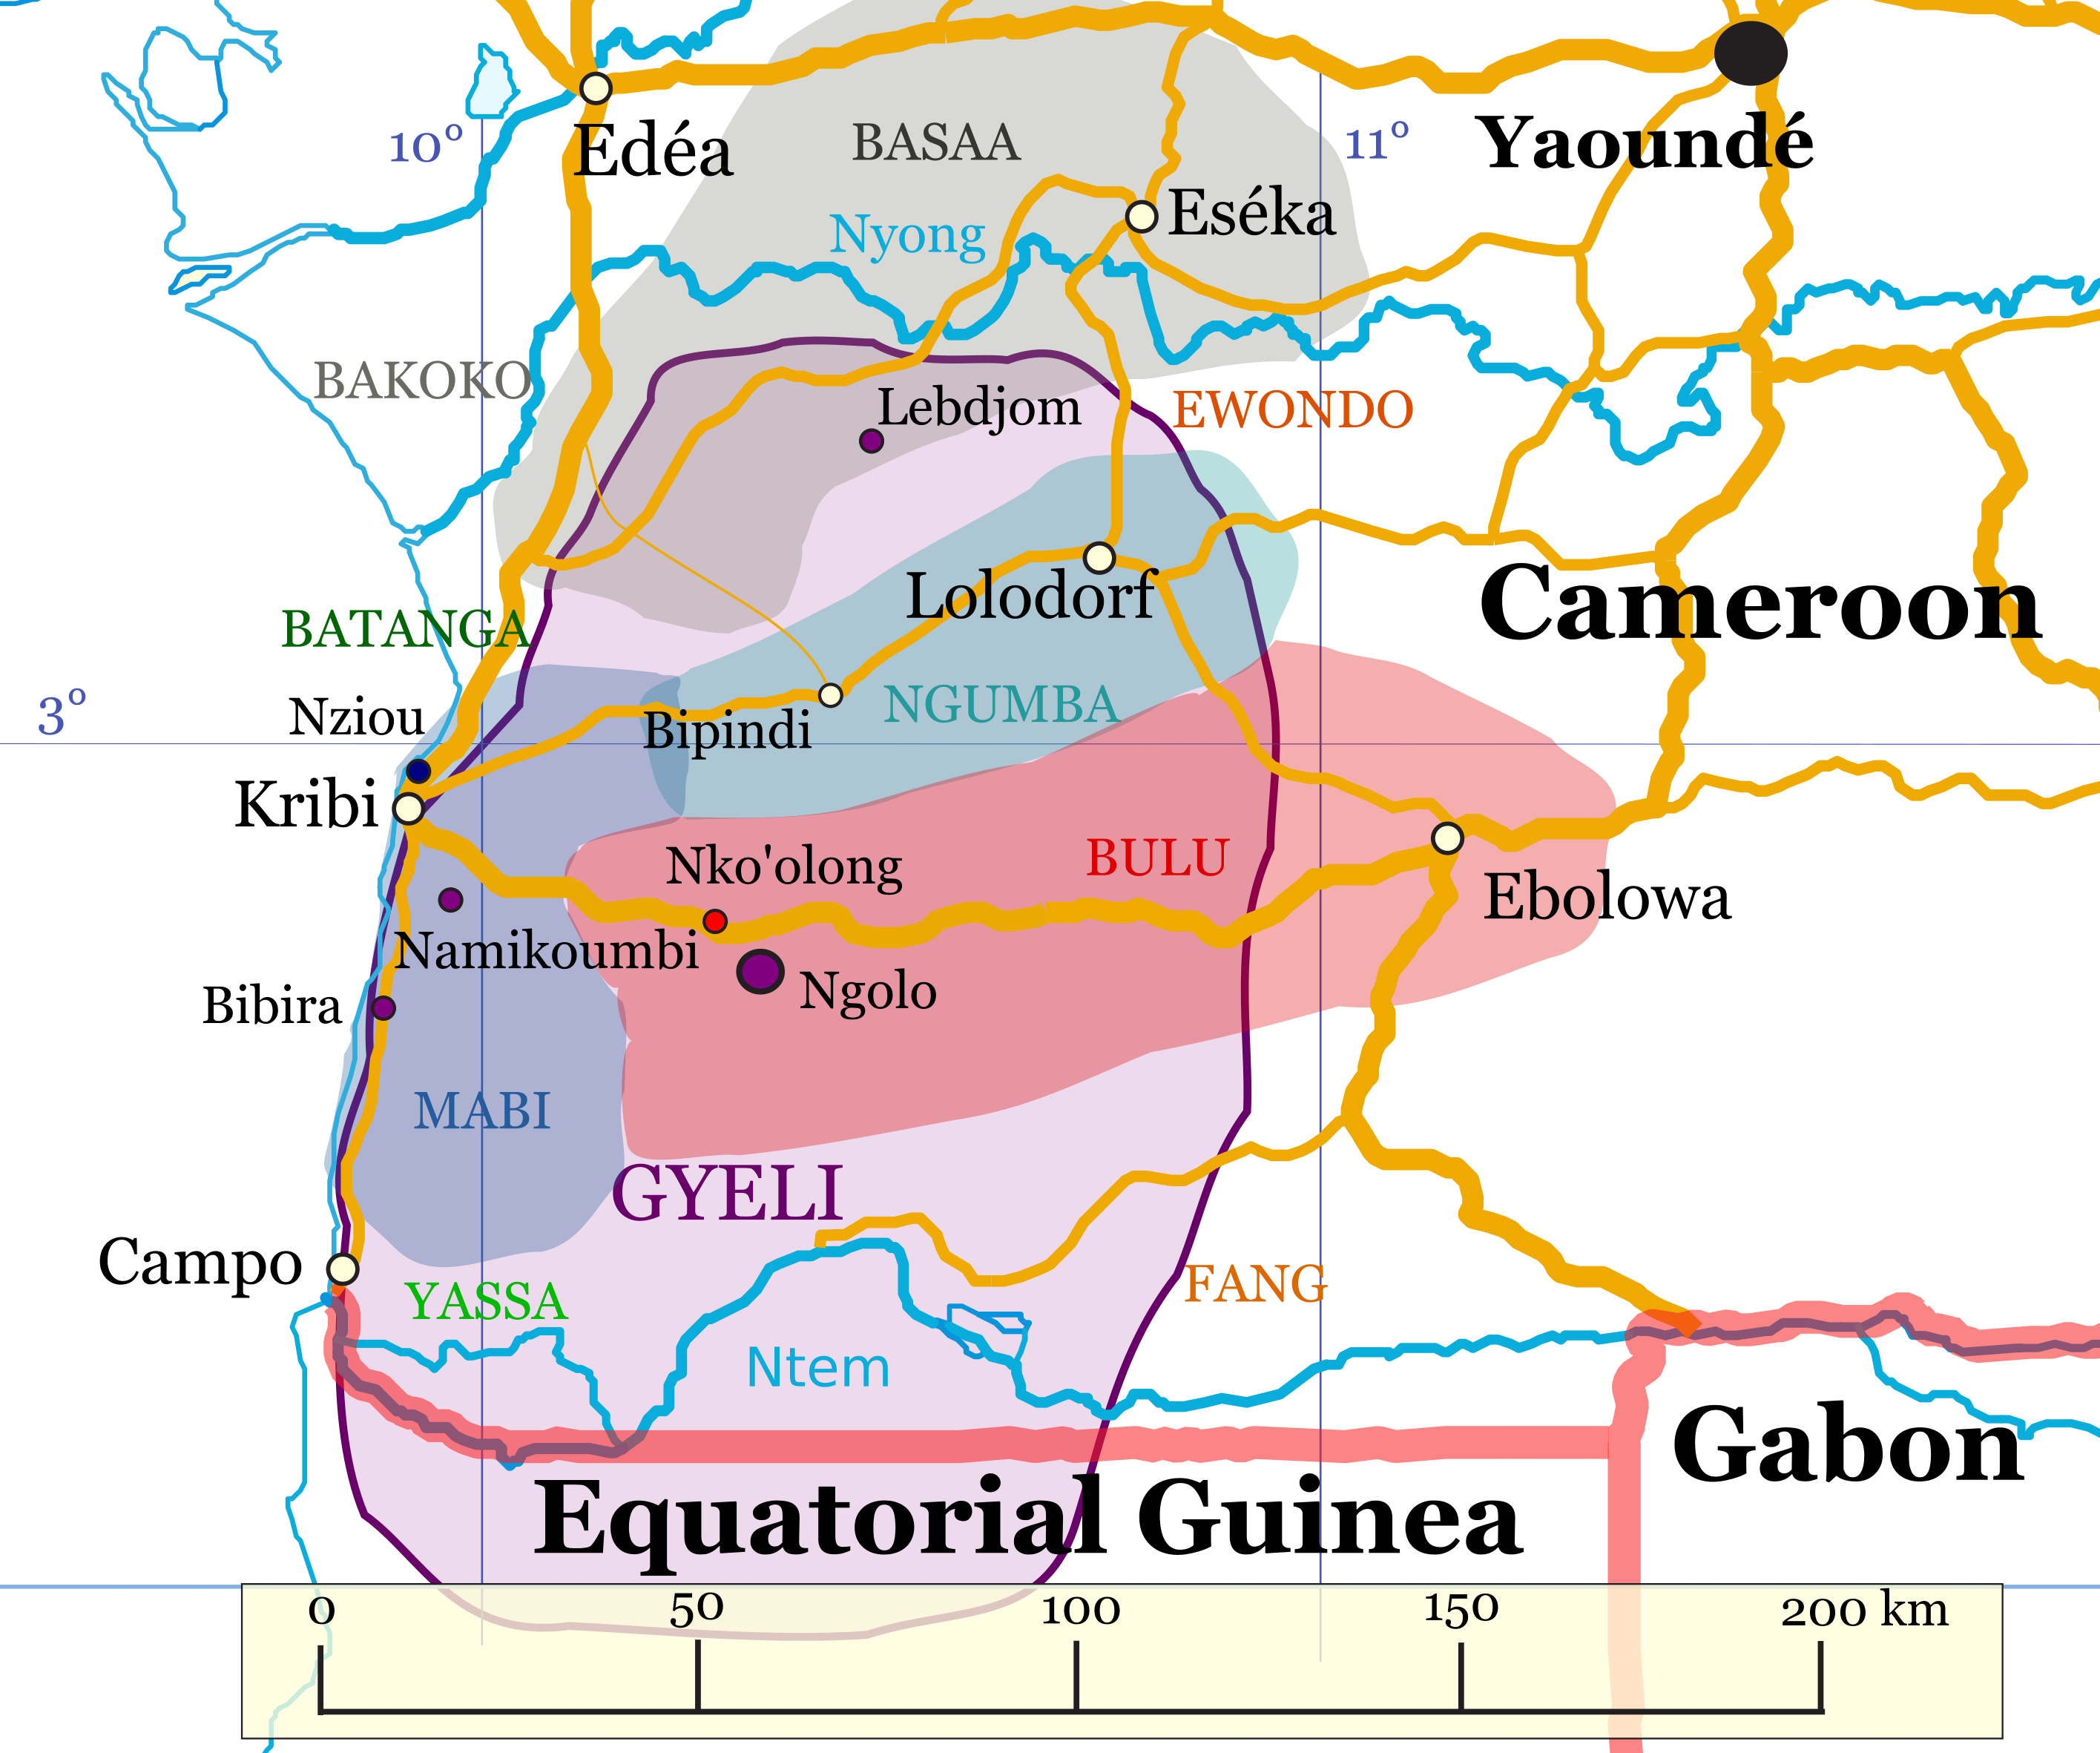
\includegraphics[width=\textwidth]{figures/Gyeli-map2021.png}
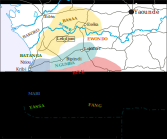
\includegraphics[width=\textwidth]{figures/gyelimap2.pdf}
\caption{Map of the Gyeli language area and its neighboring languages}
\label{Fig:Gyeli-map}
\end{figure}

It is characteristic for this part of Cameroon that languages are geographically quite interspersed. Usually, there is no clear-cut area that only contains one language. Taking a road in the northern part of the Gyeli speaking area, for instance, one might pass a Basaa village. The next village is Ewondo and then the next one is Basaa again. This is, of course, quite difficult to visualize in a map showing a surface larger than 12,500 km\textsuperscript{2}. Therefore, the map in \figref{Fig:Gyeli-map} is best understood as an approximation rather than the representation of a linguistic reality.


\subsubsection{Contact with Bantu farmer groups} 
Bantu farmer languages in contact with Gyeli include (read clockwise starting in the northwest in the map of \figref{Fig:Gyeli-map}): Batanga, Bakoko, Basaa, Ewondo, Bulu, Fang, Yasa, and Kwasio with its two dialects Mabi and Ngumba. All of these languages also belong to the Bantu A zone, though to different subgroups, as illustrated in \tabref{Tab:Contact}.\footnote{Each language name is accompanied by the ISO code as used in the {\itshape Ethnologue}.}
 
\begin{table}[t]
%\scalebox{0.95}{
\begin{tabularx}{\textwidth}{lXl}
 \lsptoprule
Group & Languages & Color in Fig. \ref{Fig:Gyeli-map} \\
 \midrule
A30 & Batanga (bnm), Yasa (yko) & green \\
A40 & Basaa (bas), Bakoko (bkh) & grey \\
A70 & Bulu (bum), Fang (fan), Ewondo (ewo) & red \\
A80 & Kwasio (nmg) with two dialects Mabi and Ngumba& blue\\
 \lspbottomrule
\end{tabularx}
\caption{Classification of Gyeli's contact languages}
\label{Tab:Contact}
\end{table}

The nature of contact and thus the linguistic closeness between the Bagyeli and speakers of these eight different farmer groups differs depending on the socio-economic relations in play. The Bagyeli have closer relations to some farming groups than to others. Contact with the Yasa, for instance, who are traditionally fishermen, is less intense than with the Kwasio who are, at least partially, agriculturalists: the Bagyeli seem to be more interested in agricultural products than in seafood. There may also be historic reasons why relations to some farming Bantu groups are closer than to others depending on whom the Bagyeli had first contact with and which Bantu farmer groups arrived later in the area. Further, on an individual rather than a group level, the type of contact may be different between individual Gyeli and farmer families. Some Gyeli families have closer ties to certain farmer families than others. 

The picture is thus quite heterogeneous and would require a thorough socio-economic survey supplemented by historical information in order to provide a more informed account of the nature of different types of contact. Since such a survey for the whole Gyeli speaking area would exceed the frame of this work, information presented here is based on statements by my informants, both Bagyeli and farmers, on sociolinguistic information gathered in the Gyeli village Ngolo, and on my observations of contact behavior between some Gyeli and farmer groups.

It is important to keep in mind that the status of Gyeli and the surrounding farmer languages are not the same concerning the prestige of the languages. Gyeli is associated with backwardness, a lack of education and even civilization. The Bantu farmer languages, in contrast, are the languages of the Bagyeli's patrons, associated with power and prestige. Thus, in inter-ethnic communication between Bagyeli and Bantu farmers, it is the farmers' languages that are being used. In fact, the farmers do not speak Gyeli. If some farmers understand snippets of a conversation among the Bagyeli this is only due to a certain amount of linguistic similarity between Gyeli and Kwasio.




\subsubsection{Multilingualism} 
Speakers of all different languages in the area are in contact with some other languages; it is not only the Bagyeli being in contact with Bantu farmers. As a consequence of this close contact as well as intermarriage and trading relations, just to mention the most important factors, members of all ethnic groups are multilingual. This also holds for the Bagyeli who are multilingual with at least the three languages they speak, but usually even more. How many and which languages a Gyeli speaker masters depends on the location of his or her village within the Gyeli speaking area. Given the geographic size of the Gyeli speaking area, it is obvious that a single Gyeli speaker is not in contact with all of the eight contact languages. Rather, Gyeli speakers are in close contact with usually one main contact language. Further, all Bagyeli seem to speak or at least understand Kwasio, Gyeli's closest linguistic relative. Whether a Gyeli speaker speaks other languages than Kwasio and potentially another language of close contact depends highly on individual ties to other Gyeli groups and individual mobility. For instance, if a Gyeli speaker from a village in the Bulu contact area has relatives in another Gyeli village closer to the Fang contact area where he or she spends a certain amount of time, he or she will likely pick up some of the Fang language.

Of course, it is difficult to measure the degree of fluency in several languages of even a restricted number of Gyeli speakers given the number of languages the Bagyeli speak and the various factors for acquiring contact languages. Since it was not possible to test fluency of all the various languages my consultants claim to ``speak'', information provided here relies to a large degree on the speakers' self-assessment, at least for those languages I have not witnessed interactions with. In the case of Kwasio and Bulu, I was able to observe communications with the respective farmers and I am sure that the Bagyeli indeed speak these languages they claim to speak. For other languages, however, I do not have any data based on observation. In any case, the Bagyeli I have worked with have a good intuition of the languages of the area, even of those they do not speak: playing Gyeli texts from other contact regions to them, they were able with a high degree of accuracy to detect loanwords from other contact languages within the text and, even though they did not understand the meaning, they were able to indicate the source language. 


While Gyeli is in contact with several Bantu farmer languages, there is also contact between  different Gyeli varieties which I will describe in \sectref{sec:dialects}. Bagyeli of the Bulu contact area also have strong ties with other Bagyeli in the Mabi contact region who speak a different dialect. Contact among Bagyeli of different contact languages may be the primary reason that speakers have such a good intuition about languages of the area, even if they do not speak them.


\subsubsection{The role of French} 
The last element in Gyeli's language contact situation is the colonial language French. Gyeli is not (yet) directly influenced by French. Many Bagyeli do not go to school and thus do not speak French. This situation, however, may change rapidly since more schools are being built and the government, as well as some NGOs, make an effort to facilitate schooling for Bagyeli children. Nonetheless, Gyeli speakers already use a few French words that regularly show up in texts. These  words include mostly particles and filling words such as {\itshape donc} `so', {\itshape alors} `well' or {\itshape allez} `let's go' and seem to have the emblematic function of showing a certain education. They are borrowed from Bantu farmers who use the same expressions in code-switching in their languages for exactly the same purpose.

\subsubsection{Language contact situation in Ngolo} 
Ngolo is situated in the Bulu (A70) contact area, so Bulu is the primary farmer language of influence. The Bagyeli in Ngolo are all multilingual. Besides Gyeli and the main contact language Bulu, they also speak Kwasio (A80) (mostly its dialect Mabi, but some speakers rather speak the other dialect Ngumba). Further, most consultants in Ngolo speak Fang (A70). A few speakers in Ngolo have traveled far and state that they speak even Makaa, Eton and Bamenda. %Even though I did not test their level of fluency, it seems trustworthy that they have at least some basic knowledge of these languages.

Concerning the command of French, the Bagyeli in Ngolo have a comparatively good school education. In contrast to many other Gyeli villages, their children have attended school more or less regularly for a couple of years. Further, some of them have worked in the nearby rubber plantations where they had to interact in French. Thus, they all speak French on a basic level. Their command is, however, not enough to have a whole conversation or even do elicitations in French. There is a general tendency that Gyeli speakers in Ngolo rather understate their level of French by claiming that they do not speak French at all, while it turns out that they actually do speak some and they definitely understand more than they claim. 

In terms of contact with other Gyeli varieties, the main contact dialects include Gyeli as it is spoken in contact with Mabi and Ngumba. Further, inhabitants of Ngolo are in contact with Gyeli villages in the Fang region. Since our project did not gather data in this region, however, it is not clear whether the Gyeli variety of the Fang region constitutes a different dialect than the one in the Bulu region. On an individual level, family ties may reach further than these regions. 

As a consequence of all these factors, there is a high degree of linguistic variation even within just one village, depending on a speaker's individual linguistic background.
In intra-ethnic communication, every Gyeli speaker just speaks their idiolect and everybody understands without attempting to correct each other concerning,  for example,  phonetic realizations or lexical choices. One reason for this non-prescriptive language behavior is likely due to the fact that there is no standard variety which could serve as the norm.  Other factors may include a low level of education and a relatively egalitarian social system. An extreme example in Ngolo concerns a Gyeli woman who grew up with Kwasio farmers and thus speaks Kwasio even after having returned to the Gyeli village. This does not seem to bother the other Bagyeli who speak Gyeli with her while she keeps speaking Kwasio. 


\subsection{Dialects}
\label{sec:dialects}

Gyeli speakers are currently shifting to the languages they are most closely in contact with, due to massive changes in their environment, as outlined in \sectref{sec:LangEnd}. In the course of this language shift, different Gyeli dialects are emerging, as previous work and results of the current DoBeS project (\sectref{sec:Dobes}) show. 

Already in the 1970s, \citet[29]{renaud76} noticed two varieties, based on phonological, morphological, and lexical differences. He refers to one variety as  ``Bajele'' which he views as more innovative, while the ``Bakola'' variety is said to be more conservative, being more closely related to Proto-Bantu than to the Makaa-Njem group.\footnote{This generalization is based on only 221 lexical items. It is also not quite clear what the innovative versus conservative features are specifically.} He further states that both varieties are mutually intelligible and not bound to any specific geographic distribution.

While it is true that Gyeli varieties are mutually intelligible, there seems to be some geographic distribution which is linked to Gyeli's contact languages. Renaud's ``Bakola'' variety seems to roughly correspond with Gyeli as spoken in the Basaa contact area, while his ``Bajele'' variety refers to the dialect spoken in the Ngumba contact area.\footnote{A reason why Renaud does not notice any particular geographic distribution of the two varieties may be due to his fieldwork location around Bipindi (see \figref{Fig:Gyeli-map}). Bipindi lies at the intersection of two roads: along the east-west road, there are mainly Ngumba villages, while the road to the north houses many Basaa villages. Nevertheless, villages of different ethnic groups are generally interspersed and there is lots of contact between all groups. In addition to that, the Bagyeli are highly mobile and frequently stay in other Gyeli villages. Therefore, it is not surprising that both names seem to be used interchangeably within the same area.}
It seems, however, misleading to assume two varieties based on the two different names for the Gyeli language.  Rather, there are more varieties than just two, but none of them have a specific name, neither given by the Bagyeli nor by outsiders. The terms ``Bakola'' and ``Bajele'' are originally exonyms from Basaa and Kwasio, respectively, which have become endonyms in the different Gyeli varieties and other Gyeli varieties. 

The data from the DoBeS project on Bakola/Bagyeli suggests that there are at least three dialects: one that is influenced by Basaa, one by Kwasio, and the third by Bulu. There may be more dialects corresponding to other contact languages, such as Fang or Bakoko. Given the vast geographical area and number of contact languages, it was, however, beyond the frame of the project to investigate potential dialects in the entire Gyeli speaking area. Additionally, linguistic variation within the language is not classified by speakers by different dialect names. Thus, speakers would acknowledge that other Gyeli speakers speak ``differently'', being more influenced by a certain contact language, but there is no systematic classification nor labelling of varieties. 
As such, it is difficult to artificially label different varieties. Further, the geographic extent of a certain dialect is not  known exactly at this point and must be taken as preliminary.

Therefore, we do not suggest any specific names for different Gyeli varieties, but rather refer to roughly where a dialect is  spoken (not specifying the exact geographical extent). Within the three different contact regions that we investigated, namely Kwasio, Basaa, and Bulu, we collected data from several locations. This way, we made sure that the language variety is not only spoken in a particular village, but in a broader region.

Dialectal differences as observed within the DoBeS project are based on phonological and lexical differences. For instance, while the Gyeli variety that is primarily in contact with Bulu uses alveolar fricatives [s] and [z], these are systematically realized as postalveolar fricatives [ʃ] and [ʒ] in the Kwasio contact region. Another example concerns voiced bilabial and dental implosives which occur in the dialect that is in closest contact with Basaa, but which are lacking in the varieties of the Kwasio and Bulu contact region. Lexically speaking, each variety has a number of loanwords from its closest contact language that lack in different varieties.

Since the goal of this work is a grammatical description of one of the Gyeli varieties, an
exact dialect comparison with a more extensive list of distinguishing features has to wait for future research, as well as determining more precisely how many Gyeli varieties there are. Another question that cannot be answered at this point concerns the historical development of Gyeli dialects. Thus, it is currently not clear when different varieties started to emerge and whether this ties in with sedentarization patterns or whether dialectal differentiation started already before the Bagyeli became sedentary as of the 1960s.\footnote{This date is given by \citet[25]{renaud76}.}



\subsection{Language endangerment}
\label{sec:LangEnd}

Gyeli is considered an endangered language. 
Symptoms of Gyeli's status as an endangered language include a high level of bilingualism and on-going adaptation of the native languages of neighboring Bantu farmers. Other factors that are usually taken as signs of language endangerment such as low speaker numbers and a low level of transmission to the young generation seem to be less indicative. Currently, there are about 4,000 to 5,000 Gyeli speakers. While this is not a high number in comparison to larger languages in the world, the number is not alarming {\itshape per se}, given that all members of the ethnic group speak the language. In addition, the language is still passed on to Gyeli children and it seems that the current young generation is still fully fluent in Gyeli.

All Bagyeli are, however, at least bilingual with an increasing amount of situations where they use the non-native language. As a result, the non-native language has an impact on the way Gyeli is spoken, as outlined in \sectref{sec:dialects}. Investigating the causes for the increased use of other languages than Gyeli reveals the level of endangerment, even though this is not (yet) reflected in speaker numbers and language transmission to the next generation.

The two major causes for Gyeli to be viewed as endangered concern massive changes in the Bagyeli's environment, as discussed in \sectref{sec:Environ}, and the low social status of the Bagyeli. While the Bagyeli are traditionally hunter-gatherers depending on the forest for food resources, they are increasingly forced to change their subsistence strategy towards more sedentary farming activities.
Together with this economic change, they are also linguistically adapting to their farming neighbors.

Another factor that reinforces language endangerment is the low prestige of Gyeli which ties in with the low social status of the Bagyeli as an ethnic group within the Cameroonian society. The Bagyeli are discriminated against by other Bantu farmer groups for their  perceived backwardness, ``primitive'' lifestyle, low level of education, and lack of political organization and thus power. While not all Bantu farmers have a negative attitude towards the Bagyeli, the general sense is that the Bagyeli need to change their lifestyle, become sedentary and modern, educated and part of the general Cameroonian society. 

Such expectations as well as discrimination have an impact on the Bagyeli's linguistic behavior.  As \citet[218]{ngima2001} notes,  Bagyeli reportedly prefer to speak Kwasio when addressing outsiders. Since language also has an emblematic function, many Bagyeli prefer not to speak Gyeli to outsiders since they perceive their language as a sign of their putative backwardness. Instead, speaking a Bantu farmer language shows a higher level of education and distances the speaker less from the other Cameroonians. This was confirmed in my fieldwork experience, speakers had an initial tendency to switch to Bulu or Kwasio when speaking with the interpreters until they got used to speaking their language with outsiders.

Given the massive environmental changes in the area as well as the enormous social pressure to adapt to the Bantu farmers' lifestyle, it seems just a natural consequence to also adopt linguistic practices. Therefore, the future of the Gyeli language is far from being safe, despite current fluency amongst Gyeli children.

%There are two factors that reinforce its endangerment. The first one concerns the social status of the Bagyeli among their neighbors and within the Cameroonian society. The Bagyeli report that they are discriminated against by the farming populations because of their “primitive” lifestyle as hunter-gatherers, as it is perceived by the farmers, their poverty, and lack of education. These negative aspects are also attributed to the language. Thus, the language is used strictly for in-group communication and usually not spoken in public when outsiders are present (Duke, personal experience). When asked what language they speak, the Bagyeli name the language of the villagers. They often even deny that they have a separate language of their own (Duke, personal experience). 

%The second factor concerns the Bagyeli's decreasing ability to continue their traditional lifestyle. Due to massive changes in their environment such as the construction of the biggest port in Central Africa, deforestation, expansion of palm oil plantations and the construction of more and more roads, the animals that the Bagyeli depend on, disappear. As a result, they are forced to change their subsistence strategy, become sedentary and adapt more and more to a farming lifestyle. In the course of these changes, the Bagyeli adapt to their neighbors who are already farmers and have more prestige than the hunter-gatherers, and shift to their languages.

%The construction of the port has a big impact on some of the Gyeli villages. The village Bibira was relocated in spring 2012 to make way for the construction site. Before the relocation, the Bagyeli in Bibira lived right next to the road where trucks were passing every few minutes for many months. Their “new” Bibira consists of three wooden houses the Bagyeli are very proud of on a patch of former rain forest. The Bibira inhabitants report, however, that skin diseases have become more of a problem since they left the forest. They also worry that they will be relocated soon again because their new village is only temporary – the government has not yet found a permanent place for them.

\subsection{Special features of Gyeli}


In terms of its linguistic structure, Gyeli yields features that are of interest to both Bantuists and to general typologists. In the following, I will list a few examples. 
Phonologically, for instance, Gyeli has more complex consonants and consonant clusters than other Bantu languages. These include, for example, homorganic affricates /pf/ and /bv/ and the prenasalized labio-velar /mgb/. Sounds that are usually analyzed as implosives in neighboring languages are realized as pre-glottalized and prevoiced stops in Gyeli.

Gyeli has a very complex tone system since tone plays a central role in this language, both for lexical distinctions and grammatical functions. Tense-mood distinctions are achieved without segmental morphemes, but only by tonal manipulation of  the subject-clause-operator (SCOP) and the tonal pattern of the verb. In addition to tense-mood marking, tone also has a syntactic function of linking the closest argument to the verb. Tonal processes differ between the nominal domain, where high tone spreading goes from left to right, and the verbal domain where high tones spread from right to left.

In terms of nominal morphology, Gyeli has a remarkable system of genitive constructions when linking two nouns via an attributive marker. While the mar\-   ker generally agrees in gender with the head noun, it receives a special form when the head noun is a proper name. Besides, Gyeli has intricate rules under which the attributive marker can be omitted in contrast to contexts when it has to occur.

Another typologically rare property of Gyeli concerns its postpositions. As \citet{dryer2013a} shows, languages with a basic V O word order usually have prepositions. While Gyeli has a basic V O word order, it  nevertheless has both pre- and postpositions.

While Bantu languages are generally known for their productive verb extensions, part of the Gyeli verbal derivation system is being simplified, merging applicative and causative suffixes. In contrast, the language has an elaborate system of lesser studied extensions, distinguishing for example autocausatives and positionals.

Gyeli also has a rich system in terms of negation strategies. The expression of negation depends on the tense-mood category and clause type. While in the \textsc{present} negation is marked by a suffix on the verb and a special tonal pattern of the \textsc{stamp} clitic, negation in \textsc{past} and \textsc{future} is encoded by distinct negation words. The \textsc{present} as well as subordinate clauses further use a negation adverb which requires an infinitival verb in dependent clauses.

%The language has a multitude of ways to express non-verbal predicates, using three different non-verbal copulas and three verbal forms. The choice of the form depends both on the tense-mood category of the phrase and the type of relation between the subject and the non-verbal predicate.


\subsection{Previous literature}
\largerpage
Languages of the Makaa-Njem group are generally under-studied.
While there are a few accounts by SIL missionaries and local students, these works are often difficult to access. Probably the best known and widely available description of an A80 language is the sketch grammar on Makaa by \citet{heath2003}.  \citet{cheucle2014} provides a thorough comparative study of the A80 languages, comparing phoneme and tonal inventories as well as noun class systems. She also gives a valuable review of the linguistic literature of the Makaa-Njem languages so that I will not go into further detail here in this respect. Instead, I will review the existent literature on Gyeli, both linguistic and non-linguistic.

Previous linguistic literature on the Gyeli language is quite limited. It includes a description of ``Bajɛle'' by \citet{renaud76}. This work is quite valuable and detailed in many respects. It is, however, restricted to the phonology and nominal morphology of the Gyeli variety that is spoken around Bipindi in the Kwasio contact region (with some influence by Basaa).
Therefore, the description of the Gyeli variety spoken in Ngolo extents Renaud's work in terms of a more in-depth grammatical description, covering, for instance, also verb morphology and clause types. It further adds to our knowledge about Gyeli varieties, given that the variety spoken in Ngolo constitutes a different dialect in comparison to the variety that Renaud studied. 
An additional resource is   \citet{letouzey75} which provides an ethnobotanic perspective on the language by comparing Gyeli tree names with other languages of the region.

Early publications on the Bagyeli  come mostly from missionary and traveller reports. This is, for example, the case with \citet{seiwert26} who gives an anecdotal account of his encounters with the Bagyeli in {\itshape Anthropos}. Other reports had been published even before the turn of the 20th century in German colonial reports and ethnographic journals. A list of these very early publications on Gyeli, which are generally difficult to get access to, is provided in \citet[357-360]{renaud76}. 
Newer ethnographic publications on the Bagyeli include papers by, for example, \citet{joiris94} and \citet{ngima2001} which both focus on the relationship between the Bakola and their neighbors. 
While this list is certainly not exhaustive, it covers the seemingly most important ethnographic studies, supplementing Renaud's list.

Recent years have also seen a flourishing literature involving research on the Bagyeli in other scientific areas. One domain of publications involves ethnopharmacological and medical literature. \citet{fomogne2014},  for instance, investigate the Bagyeli's plant use for treating respiratory problems.  \citet{mauclere2011} study viral infections in the Bagyeli population as compared to the Bantu farmer population.

Another area of great attention in the recent literature concerns  the Bagyeli's changing environment and their (lack of) protection as an ethnic minority group. For instance, \citet{pelican2009} discusses the impact (or lack thereof) of the Declaration on the Rights of Indigenous Peoples by the United Nations General Assembly in 2007 on ethnic minority groups such as the Bagyeli in {\itshape American Ethnologist Journal}. \citet{germond2012} explores discourse dynamics in the construction of indigenous peoples by different actors of conflicting interests in the {\itshape International Journal on Minority and Group Rights}. The impacts of the developing oil industry in the Gyeli speaking area are investigated in {\itshape Cultural Survival Quarterly} by \citet{nelson2004} and in the {\itshape Journal of Developing Societies} by \citet{swing2012}. 

In addition to traditionally published resources, more information on the Bagyeli is also found in other media, for example online. The DoBeS language documentation project that constitutes the framework of this description (see \sectref{sec:Dobes}) provides information along with pictures and links to audio and video recordings in the DoBeS archive.  Another online source is provided by the anthropologist \citet{devin2015} who has a website on different Central African ``Pygmy'' groups online, including information on the Bagyeli/Bakola. Further, there are various documentaries. \citet{lorenz2014} produced a documentary series in three episodes as part of our documentation project. Another documentary was done by \citet{thomopoulos2012}. %Finally, also {\itshape youtube} hosts a growing collection of snippets on the Bagyeli/Bakola.





\section{The Gyeli speakers}
\label{sec:GyeliSp}

In this section, I provide more information on the Gyeli speakers, including their environment and lifestyle in terms of culture and subsistence.

\subsection{Environment}
\label{sec:Environ}

Gyeli (or Kola) speakers live roughly in the area between the Nyong river in the north and the Ntem river at the border to Equatorial Guinea, as shown in the map of \figref{Fig:Gyeli-map}. \citet{lewis09} reports in the {\itshape Ethnologue} that a few Gyeli speakers also live in Equatorial Guinea, but the majority of speakers are found on the  Cameroonian side.
On a west-east axis, the Gyeli speaking area stretches from the coastline of the Atlantic Ocean to about 150km inland, not quite reaching the town Ebolowa. 

The Bagyeli are forest foragers of the tropical rainforest in southwestern Cameroon. Woodlands usually consist of primary rainforest, but also more and more of secondary forest, i.e.\ forest areas which have regrown after logging.
Primary rainforest is also increasingly replaced by private gardens and manioc farms and industrial plantations for rubber, cocoa, and palm oil.

Generally, forest areas are still large, however, and often difficult to access since roads are few and often so bad that they cannot be used by cars. Also, the rainforest is interspersed by a multitude of waterways, rivers, streams, and creeks. These could potentially be used as infrastructure through the forest, but the Bagyeli usually walk by foot rather than building canoes to use these waterways for moving in the forest. The same is true for the Bagyeli who live close to the coastline: canoes are not part of their transportation system.

The climate in this part of the world is tropical with an alternation of dry and rainy seasons. There is a dry season from November through February with temperatures reaching 32 degrees Celsius. March through June is a so-called ``small'' rainy season with drizzly rain while July is relatively drier again, but generally cooler than the big dry season. June and July are usually the busiest times of the year for the Bagyeli since this is the season for intensely collecting honey, fruit and nuts. The time from August through October receives most of the precipitation in a year with almost daily strong rains and heavy storms.


%The reason for this forced change is an increased deforestation in the whole region which deprives the Bagyeli of the animals and plants they depend on in the forest. Massive deforestation is currently accelerated by a multitude of factors: logging companies destroying the rain forest in search of tropical woods,  large amounts of primary forest being replaced by palm oil and rubber plantations. Other  industrial and infrastructure developments also diminish forest areas. For instance, an oil pipeline cross-cuts the rain forest, running from Chad to the shore off Kribi. At the same location, the biggest port for central Africa was built in the last five years, starting in 2010 and being inaugurated in 2015. The port requires more infrastructure development inlands in order to ship goods to and from the port. Thus, the construction of roads and railroads is anticipated, diminishing the rain forest further. The long-term demographic  changes that the new port will bring to the region are still not fully predictable, but inhabitants of Kribi foresee that their town will grow to a dimension such as the metropolitan area of Douala, becoming economically even more important. In any case, this development leaves no room for a tradition forest forager lifestyle and the Bagyeli must adapt to the new circumstances.

While the Bagyeli live traditionally as mobile hunter-gatherers in the rainforest, the changing landscape of the last decades is one cause for changes in their lifestyle. A lot of Gyeli villages are now also found alongside roads in close vicinity to Bantu farmer villages. Those who do not live close to the roads usually stay in more remote areas. These remote areas are typically regions that are less valued by the Bantu neighbors for their farming activities, such as hill sides, wetlands or the immediate area around protected forest such as the Campo Ma'an Reserve. 

As a general tendency, there are fewer and fewer places the Bagyeli can live in the forest because of rapid deforestation. Industrial development of the region has the biggest impact on forest destruction. Forest area is significantly decimated by the construction of the deep-sea port south of Kribi, the largest port for central Africa which was inaugurated in 2015. The Kribi port complex spreads over 26,000ha and a coastline of 20km, according to \citet{ntaryike2015}.  Related infrastructure development projects further cause forest loss, such as the oil pipeline that runs from the border of Chad to the new port. The port also requires an extension of the existing road and railroad net for inland transportation. \figref{Fig:Gyeli-env}\footnote{Thanks to Sebastian Nordhoff for reworking an earlier version of this map.} shows some of the landscape  changes, including protected forests, the new deep-sea port, and the oil pipeline.

\begin{figure}
% 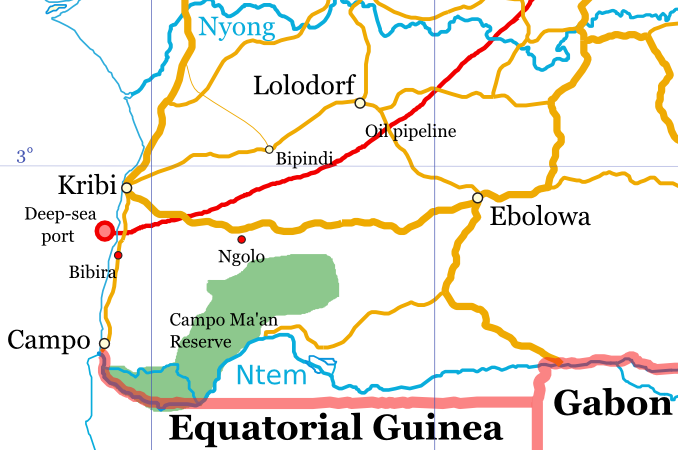
\includegraphics[width=\textwidth]{figures/Gyeli-env.png}
\includegraphics[width=\textwidth]{figures/gyelimap-landscape-changes.pdf}
\caption{Map of landscape changes in the Gyeli area}
\label{Fig:Gyeli-env}
\end{figure}

\newpage
Other manners of land exploitation also deprive the Bagyeli of rainforest areas they formerly had access to. 
There have been increased logging activities for tropical woods. Industrial plantations such as SOCAPALM (palm oil) and  HEVECAM (rubber) take over and expand on former primary rainforest.\footnote{Both plantations are roughly located to the southwest of Ngolo, but it was impossible to find any maps of their extent. Information on their total surface is also difficult to find. In a project approved in 1980, the \citet{worldbank2015} specifies that the HEVECAM rubber plantation has a surface of 40,000ha. These figures are, however, most likely outdated, while exact figures for SOCAPALM do not seem to be publicly accessible. For a general overview, the \citet{worldres2015} provides more systematic information on the kinds of land use in the Forest Atlas of Cameroon. It is, however, not always clear who has the land rights.} Even projects that are intended to protect the environment, such as the Campo Ma'an Reserve, displace the Bagyeli from former areas they inhabited since they are not allowed to live within the Reserve.

%map?  Campo Ma'an, Kribi, Ngolo, industrial plantations such as SOCAPALM (palm oil) and  HEVECAM (rubber) plantations?

%All these environmental changes ultimately lead to a loss of land and food resources. As a consequence, the Bagyeli are forced to  increasingly adopt farming strategies in order to make a living.  


\subsection{Subsistence and culture}
\label{sec:Cult}


\subsubsection*{Subsistence} The Bagyeli are traditionally forest foragers who live off hunting animals in the rainforest and gathering plants, fruit, nuts, and honey. Hunting techniques involve killing animals with spears and machetes as well as net hunts with a larger group of individuals. Every Gyeli village has a number of dogs that help with hunting. The Bagyeli also build different types of traps, depending on the animal they are looking for. Animals that the Bagyeli eat include all sorts of monkeys, wild cats, different types of antelopes ranging from small duikers to larger water bucks, mongooses, bush rats, porcupines, as well as snakes and snails.

Fish is also on the dietary plan, but is less valued than meat. Fishing is regarded as a pastime, especially for children, but not as a serious activity. Bagyeli catch fish in creeks in the forest by building dams or, in deeper rivers and the sea, by using fish lines, standing on rocks. All of them are usually good swimmers, but they do not venture out into the sea.

Honey is highly valued for it is often dangerous to reach. Bee hives are usually high up in trees so that the Bagyeli have to climb a tree and smoke the bees out -- without any security line holding them.
Vegetarian food resources involve different types of tubers, fruit that grow in the forest, such as the so-called wild mango that is used to make a sauce, and nuts. 

Since primary forest is becoming increasingly scarce, so are the animals and plants the Bagyeli depend on. Therefore, the Bagyeli get more and more engaged in other activities as well in order to make a living.  This concerns foremost low-scale farming such as growing fruit trees (e.g.\ bananas and plantains, bread fruit, {\itshape Dacryodes edulis}, known as African pear or plum trees), which require little maintenance. They also grow other plants which need more care in small fields, such as manioc and yams. Keeping chickens is another innovation in many Gyeli camps.

Besides farming activities, some Bagyeli may earn a little bit of money through day labor in the industrial plantations or with the Bantu farmer neighbors and through selling wild meat and baskets they make. A few villages have also discovered tourism as a source of income where they take gifts (money, food, drinks) in return for pictures the tourists take.

\newpage
\subsubsection*{Sedentarization and mobility patterns}
While the Bagyeli were traditionally nomads, who changed their camp sites frequently, they have become more and more sedentarized over the past decades\footnote{\citet[25]{renaud76} assumes progressive sedentarization since the 1960s, while \citet[86]{joiris94} proposes that the Bagyeli have become increasingly sedentary already since the early 1900s.} as a result of environmental changes as well as government efforts. As a consequence, Gyeli villages are generally as permanent now as those of the Bantu farmers in the sense that the material village does not change location.

The Bagyeli do keep, however, certain mobility patterns on both a group and an individual level. Groups of Bagyeli still leave their permanent village for hunting trips that can take up several days and even weeks. On such hunting trips, the Bagyeli construct traditional huts or use seasonal camps in the forest to sleep.  Additionally, mobility is kept on an individual basis where single people move between different villages to visit relatives, partners, and friends. Such visits can also be extended to several days and weeks.


\subsubsection*{Settlement patterns}
Traditionally, the Bagyeli lived in temporary camps in the forest. The huts they used for shelter were made out of sticks and leafage. These huts are easy to assemble, requiring about 3 hours of work load.
Nowadays, many Gyeli villages are comparable to those of the Bantu farmer neighbors, with the exception that they are usually smaller in size. An average Gyeli village, of which there are more than 100 in the whole Gyeli speaking area, has 20-30 inhabitants. There are, however, also smaller settlements with just a core family of 4-5 people, or exceptionally large villages with up to 150 inhabitants.
Houses in permanent Gyeli villages are either made from wooden planks or clay, so-called {\itshape poto-poto} houses, which are highly valued by the Bagyeli since they are in the same style as the Bantu farmers' houses.
Gyeli villages are either along the roads that cross-cut the rainforest, being built in close vicinity to Bantu farmer villages, or remotely located in the forest.

Due to environmental changes, there have been recent cases of resettlement. For example, Gyeli villages that were formerly located in the Campo Ma'an Reserve were moved outside the Reserve. Now, they line the border to the Park. There are also villages that needed to make way for the deep-sea port south of Kribi, as for example the village Bibira in \figref{Fig:Gyeli-env}. While Bantu farmer villages, which were moved as well, got monetary compensation, the affected Gyeli villages have not yet received their promised compensation. Instead, wooden houses were built for them outside the forest with the prospect that they may be resettled again.



\subsubsection*{Relations with Bantu farmers}
Relations between Bagyeli and their farming Bantu neighbors are complex. Generally, the Bantu farmers have a higher prestige and marriages between Bagyeli and farming neighbor communities are unilateral -- Bantu farmer men occasionally marry Gyeli women, but Bantu farmer women do not marry Gyeli men. Apart from these tendencies, the relationship between Bagyeli and Bantu farmers takes a range of forms. On the extreme ends of this spectrum, the relationship may be described as one between masters and slaves, patrons and clients, or, on the other hand, as family relations. During the project, we have witnessed Bantu farmers who stated that they owned a certain Gyeli group and that we would have to pay them money in order to see the Bagyeli. In contrast, we have also seen Bantu farmer women who referred to elderly Gyeli women as their mother whom they treated with respect.

We interviewed Bagyeli in various villages of different language contact regions about the perceived relation to their Bantu neighbors. Many of the interviewees stated that they felt discriminated against in several ways. Discrimination, according to them, ranges from unequal treatment in business transactions to verbal and physical violence. For instance when selling bush meat, the Bagyeli would be paid much lower prices than Bantu vendors. In general, they state that they are poorly paid for day labor. Verbal discrimination involves either mockery, e.g.\ comparing bad habits such as getting very drunk to typical ``Pygmy'' behavior, or insults. In a few cases, Bagyeli also reported of physical violence and being beaten by Bantu farmers (the exact circumstances were not described). In contrast, some speakers also talked about their ``Bulu father'' who would lend them his gun in order to help young men out. This way, the young men could kill and sell more animals to save money for the required bride-price of the women they intended to marry.

In order to obtain a more holistic picture of the heterogeneous relations between Bagyeli and farmers, we also interviewed several villagers from various Bantu farmer groups. Also in these interviews, different attitudes were reflected. Some interviewees saw the Bagyeli as backward, dirty, dishonest, and ``primitive''. Many requested that the government needed to help them so that they would reach an equal development state as the farmers by building schools and hospitals. Others called the Bagyeli their ``brothers'' who were basically of equal rank. In some cases, Bantu farmers expressed great admiration for the Bagyeli's skills as dancers and healers. For example, Bagyeli are frequently invited to the farmers for weddings and funerals in order to make music and dance. Bantu farmers also consult Gyeli healers for health issues. As such, they are admired for their magical powers, but also feared.
No matter whether the attitude was more on the friendly or discriminatory side, the overall view was that the Bagyeli needed to stop living in the forest, and instead become modern people, more like the farmers themselves. 

%On a governmental (and UN) level, the Bagyeli are officially categorized as an indigenous minority group ({\itshape peuple autochtone}) that needs protection. As such, they receive special attention in some ways, but that does not generally enhance their rights nor does it improve their living conditions.In an attempt to implement the `United Nations Declaration on the Rights of Indigenous Peoples' from 2008, signs in front of some Gyeli villages, especially the more touristy ones such as Namikoumbi, now label the Bagyeli as a minority group. On the {\itshape Journée Internationale des Peuples Autochtones} (International Day of Indigenous Peoples), celebrated annually on August 9\textsuperscript{th}, Bagyeli from several villages are being brought into Kribi town in order to raise awareness of minority group rights. For the festivities, the Bagyeli are given special t-shirts and food.

%While the intentions are certainly good, this also has some serious counter-productive effects in as much as it stigmatizes the Bagyeli even more and arouses jealousy among their Bantu farmer neighbors. After all, the Bantu are also indigenous peoples, but they do not receive t-shirts, food, nor special government or NGO aid. In addition, it is questionable how far these activities tackle the real problems the Bagyeli face. Instead of granting the Bagyeli land rights, land is rather sold to private companies such as SOCAPALM and HEVECAM so that their natural habitat is increasingly diminished.  These issues are both acknowledged and discussed, for instance by \citet{lecentre2014} (the United Nations Center for Human Rights and Democratie in Central Africa). During a four day long conference in 2014, `experts' visited three Gyeli villages and thereby assessed the precarious situation of the Bagyeli.   While few Bagyeli representatives seem to have participated, \citet{lecentre2014} pleads for example for better education opportunities for the Bagyeli as well as the establishment of {\itshape chefferies traditionelles} (traditional chiefdoms), ignoring the traditional egalitarian structure of the Gyeli society. It seems to be symptomatic that, while claiming to protect indigenous peoples' rights, the very same people that are allegedly protected are not even involved in the discourse.





\section{Methodology}
\label{sec:Methodology}

In this section, I describe the methodology involved in producing this grammatical description. I first outline the project that served as the framework for the grammar. I then define the ``speech community'' whose language variety I describe before I detail the data on which this grammar is based. 

\subsection{The project}
\label{sec:Dobes}

The basis for this grammar stems from 19 months of field research as a Ph.D. candidate that I conducted within the framework of the DoBeS (Documentation of Endangered Languages) project on the Bakola/Bagyeli language from March 2010 until February 2012 and during an extended project phase from March 2013 until August 2014. 
The overall goal of the project was to document aspects of the Gyeli language, concentrating on the collection and archiving of primary data. Primary data include both audio and video recordings, covering various text genres, e.g.\ conversations, interviews, traditional story telling, songs, and descriptive texts accompanying everyday activities such as hunting and hut building. A more detailed description of the data is provided in \sectref{sec:Data}. 

The project was carried out by the project director Prof. Maarten Mous and three linguists: Dr. Emmanuel Ngue Um, Daniel Duke and myself. In addition to the linguists, the project also included a professional cameraman, Christopher Lorenz. In terms of task distribution, the three linguists 
worked in different regions of the Gyeli speaking area, as represented by the shaded areas in \figref{Fig:Gyeli-map}. Ngue Um worked on describing the Kola variety spoken in the Basaa contact area, Duke mainly worked in the Kwasio contact region around Lolodorf, but also in the Gyeli village Bibira, while the variety of my description is located in the Bulu contact region. The cameraman Lorenz joined the linguists' team each year for several weeks and made high-quality video recordings in all dialectal areas.

I collected additional data on Gyeli as a collaborator in J\"urgen Bohnemeyer's NSF \#1535846 project ``Causality across languages'' (2015-2022). This enabled me to gather stimulus-based data on the expression of causal relations during another five weeks of fieldwork in 2017.


\subsection{The construction of a speech community}

A grammar is usually the description of some variety of a language spoken by a group of speakers that, in an idealized way, constitutes the speech community. In reality, however,   
there is no such thing as a ``pure'' or homogeneous speech community. A speech community that serves as the basis for a grammatical description is rather an abstraction made by the linguist. Various factors interfere with a clear-cut concept of ``speech community'', the most important ones being language contact and multilingualism in the Gyeli case.

As outlined in \sectref{sec:LangCon}, the Gyeli language situation is complex with a high degree of language contact and multilingualism. As such, idiolects may differ quite a lot from speaker to speaker, even within the same village, depending on their individual language exposure to various contact languages and personal family ties to other Gyeli villages in other language contact regions.

I consider the village Ngolo as the speech community that provides the empirical basis for this grammar. Ngolo is located in the Bulu contact region and constitutes a different dialect from Gyeli villages in the Basaa or Kwasio speaking area. I do not, however, view the Gyeli variety as spoken in Ngolo necessarily representative for all Gyeli villages in the Bulu contact region since such a generalization would require a larger data coverage of all Gyeli villages in this region.\footnote{Data gathered in another Gyeli village within the Bulu contact region, called {\itshape Bomnapenda}, suggests, however, that the variety in Ngolo and Bomnapenda constitute one dialect as opposed to other varieties in the Kwasio and Basaa regions.}

A further complication with this ``speech community'' is to delimit who exactly is a member of Ngolo and thus to pinpoint how many speakers the community has. As explained in \sectref{sec:Cult}, the Bagyeli are still highly mobile between permanent villages. Therefore, there is always fluctuation in terms of presence and absence of individuals. While the number of houses remains stable, at any given time, I would never get the exact same set and number of speakers. The village has six houses that belong to different core families. The number of inhabitants is around thirty, including children. Core families or individuals may, however, be away for some time, visiting relatives in other villages are staying in the forest on extended hunting trips. At the same time, other relatives may be visiting and staying in the Ngolo houses.  
In order to come to grips with these dynamics,  as a working definition for Gyeli speakers of Ngolo, I consider those a member of the ``speech community'' who state that that they were either born in the village or come from another village within the Bulu contact region. 



\subsection{Data}
\label{sec:Data}

Findings presented in this grammar are based both on elicitations and an extensive number of natural texts which are accessible in {\itshape The Language Archive} (http://dobes.mpi.nl/projects/bakola/). As part of a language documentation project, the documentary team collected a variety of text genres such as narratives, procedural, hortative, and descriptive texts, dialogues, conversations, and interviews, among others. These also include a wide range of everyday activities such as hunting with different techniques such as spears or nets, building traps and huts, collecting honey, building musical instruments, preparing hunted animals, dancing, healing sessions, and telling traditional and autobiographical stories.\footnote{A selection of audio and video material and their annotations can be found in the DoBeS archive. At present, 133 audio and 90 video recordings from different dialect areas are uploaded into the archive, 69 of which are annotated.}

The text corpus that specifically serves as the empirical basis for the description of the Ngolo variety in terms of distribution and frequency of forms is comprised of 3,304 words (540 intonation phrases) of high-quality annotation, distributed over three text genres, namely a folktale, a conversation between multiple speakers, and an autobiographical narrative. I annotated the texts in coordinated discussion with the Gyeli speakers. (As Gyeli speakers are not literate, they were not able to carry out annotation tasks themselves.) Discussions with speakers were also indispensable since the tonal system of Gyeli is so complex that additional double-checking and elicitations were necessary to uncover its rules. The annotated texts can be found in  \appref{sec:AppendixII}. In addition to these thorough annotations, more natural texts have been roughly annotated and/or translated. These supplementary annotations and translations include 15 different texts and snippets of texts of about 2 hours and 10 minutes in total. In addition to annotations, I use lexical databases, one for nouns and one for verbs. The noun database includes 875 entries and the verb database 377.

I also gathered experimental data based on the language of perception field manual designed at the Max-Planck Institute for Psycholinguistics. These experiments included color naming tasks\footnote{The results of this experiment are published in \citet{grimm2014}.} developed by \citet{majid2007a}, the olfactory test by \citet{majid2007b}, the taste test by \citet{senft2007} and tests on spatial orientation by \citet{levinson93} and topological relations by \citet{bowerman92}. 

The third kind of data I collected contains elicitations and questionnaires. They are comprised of approximately 1,000 audio recording sessions with an average of 10 minutes each, and in total about 167 hours.
The questionnaires I used include, for instance, questionnaires on tense-aspect-mood, question types, relative clauses, and information structure. Each questionnaire that served as a basis for my analysis is cited in the chapter where the data occurs.
While the collection of natural text and experimental tasks took place in the village of Ngolo, I supplemented these data with elicitations and questionnaires with language consultants in Kribi. %Additional translations and annotations were done outside of the village. This proved to be the most efficient way, given the constraints in Ngolo. In terms of logistics, staying in the village would have required lots of time in order to keep up with basic tasks such as charging equipment. Since the village does not have any connection to the electricity network, I would have had to bring a generator. Storing equipment would have been a problem since the houses are neither water proof nor can doors be locked. Organizing food would have been time consuming since the village is far away from any store and I did not want to burden the Bagyeli with supplying food for me, given that it is already difficult to find enough food for their families. Also in terms of general workflow, the possibility to work with one consultant at a time outside the village was the best option. This way, we were able to work longer hours since there was no distraction from other village activities or curious children. At the same time, this improved the recording quality since the background noise level was easier to monitor.

Elicitations were carried out with one or two consultants at a time, varying between five different speakers during my fieldwork. Natural text and experimental data stem from a larger pool of speakers.
The number of speakers that provided natural text from Ngolo include at least 15 adult speakers. 
Given that the approximate size of the village is 30 inhabitants, including children, this seems to cover the entire adult population. In group conversations, children were also present and so their speech was also recorded.
Some speakers were recorded more often than others, depending on their availability. While the ratio of male and female speakers is equal, men received slightly more recording time since women seemed to be generally busier with cooking while men had more time. Since basically all speakers of Ngolo were recorded, also all age groups are represented in the recordings. Adult speakers' ages range from teenagers\footnote{In the Gyeli society, adulthood starts earlier than in western societies. Thus, teenagers of around 15 years are considered as young adults. Age is generally subject to estimation since the Bagyeli usually do not know their exact age.} to elders of about 60 years.   


%Nze
%Mambi 
%Mama
%Nandtoungou
%Aminu
%Tata
%Nkolo
%Tsimbo
%Segyua
%Ada
%Angeline
%Batebe
%Piano
%Manzoo




\section{Structure of the grammar and basic grammatical features}

This section is intended to help the reader navigate the content of the grammar and understand basic grammatical features that frequently occur in example sentences.  I first outline the single chapters of the description and then provide a guide on how to read glossed examples.


\subsection{Organization of the grammar}

This grammar is generally organized from form-to-function and divided into eight chapters. After this introductory part, I describe the phonology of Gyeli in \chapref{sec:Phon}. This chapter contains a discussion of the phoneme inventory, the syllable structure as well as a description of the tonology.

\chapref{sec:POS} provides a discussion of Gyeli's parts of speech. This not only includes major word classes such as nouns and verbs and other lexical word classes (adjectives, adverbs, and ideophones), but also grammatical word classes, such as pro-forms, modifiers, adpositions, conjunctions, or extra-sentential elements.

In \chapref{sec:WordForm}, I outline word formation processes by describing the various morpheme types found in Gyeli as well as derivation and compounding.

In \chapref{sec:NP}, I explore grammatical phenomena in the noun phrase. This includes the gender and agreement system as well as different types of noun phrases, for instance noun + noun attributive constructions.

\chapref{sec:TAM} describes the verbal complex according to predicate construction types. My basic distinction is between simple predicates, which largely encode tense-mood categories, and complex predicates, which encode aspect, mood, and modality.

The last two chapters are reserved for clause types. In \chapref{sec:SC}, I investigate simple clauses, including both verbal and non-verbal predicates. I lay out the grammatical relations found in Gyeli and discuss basic word order as well as special word order constructions, for instance within the domain of information structure and questions. \chapref{sec:CC} deals with complex clauses including different types of both coordination and subordination, e.g.\ relative and adverbial clauses. 

The eight chapters are supplemented by three appendices. In \appref{sec:AppendixI}, I list the specific verb extensions for each verb in my verb database. \appref{sec:AppendixII} contains a collection of annotated natural text. \appref{sec:AppendixIII} provides a Gyeli -- English dictionary with about 1500 lexical entries. 

\subsection{A quick guide to decoding glossed examples}
\label{sec:Guide}

In this section, I provide a brief overview of the main grammatical features in Gyeli in order to help the reader decode high-frequency elements in the glosses of example sentences.

Glossed examples are usually comprised of four lines, distinguishing the surface form on the word level in the first line and morpheme breaks in the second line, which provide important information on the underlying tonal patterns. Every vowel is marked for its surface tone in the first transcription line. In the second line, some vowels have no tone marking, indicating that they are phonologically toneless. 

In terms of transcription conventions, I follow a typical Bantu notation combined with local orthographic conventions. Only in \chapref{sec:Phon} do I use IPA conventions. I list the differences between IPA notation and Gyeli transcription conventions in \tabref{Tab:notation}.

\begin{table}
\begin{tabularx}{.8\textwidth}{Xl}
\lsptoprule
IPA & Gyeli orthography \\
\midrule
palatal nasal /ɲ/ & { ny} \\
velar nasal /ŋ/ & { n}  \\
palatal glide /j/ & { y} \\
voiced affricate /dʒ/ &  { j}  \\
voiceless affricate /tʃ/ & { ts} \\
glottal stop /ʔ/ &  { '} \\
\lspbottomrule
\end{tabularx}
\caption{Notation differences between IPA and Gyeli orthography}
\label{Tab:notation}
\end{table}

Velar nasals are virtually everywhere homorganic and precede a velar plosive. There is just one exception where the velar nasal precedes /w/ in the noun {\itshape ŋwándɔ́} `manioc stick'.  In this instance, I use the IPA version to mark the difference.


Gyeli has a basic SVO word order, as shown in \REF{i}-\REF{iii}.

\ea \label{i}
\glll [Màmbì]{\capsub{S}} [à dé]{\capsub{V}} [mántúà]{\capsub{O}}\\
	{\db}Màmbì {\db}a dè-H {\db}H-ma-ntúà \\
         {\db}$\emptyset$1.{\PN} {\db}1.{\PST}1 eat-{\R} {\db}{\OBJ}.{\LINK}-ma6-mango   \\
    \trans `Mambi ate mangoes.'
\z


The verb stem is generally preceded by a ``\textsc{stamp}'' (subject-tense-aspect-mood-polarity) clitic, which encodes information about the subject person and gender agreement, tense, aspect, mood, and polarity, as seen in \REF{i}-\REF{iii} with {\itshape à}, {\itshape mɛ́}, and {\itshape bá}, respectively. While eastern and southern Bantu languages are known for their rich agglutinative morphology, often with distinct -CV- prefixes for each of these categories, Gyeli as a northwestern Bantu language displays restrictions in segmental morphemes preceding the verb stem. Conversely, Gyeli has a rich tonal morphology where the tonal combinations on the \textsc{stamp} clitic and the verb stem yield different tense-aspect-mood categories, as discussed in \chapref{sec:TAM}. H tones attaching to the right of the verb stem, as expressed by -\textsc{h} in the second line, encode the two past tenses ({\PST}1 and {\PST}2) in some environments or a realis mood in other environments. The realis mood is pervasive in example sentences and glossed as -\textsc{r}, as seen in \REF{i} through \REF{iii}.

The subject can be dropped with the subject reference only encoded through agreement of the \textsc{stamp} clitic, as in \REF{ix}.

\ea \label{ix}
\glll  [à dé]\capsub{V} [mántúà]\capsub{O}\\
	  {\db}a dè-H {\db}H-ma-ntúà\\
        {\db}1.{\PST}1 eat-{\R} {\db}{\OBJ}.{\LINK}-ma6-mango\\
    \trans `S/he ate mangoes.'
\z



The subject is rarely expressed by a pronoun. Subject pronouns (see \sectref{sec:SBJPRO}) are glossed as \textsc{sbj} to clearly distinguish them from the \textsc{stamp} clitic, especially as most subject pronouns  are segmentally identical to the \textsc{stamp} clitic of their agreement class.  The use of subject pronouns as in \REF{ixx} usually serves information structure purposes, often indicating switch-reference through the pronoun's combination with the contrastive marker -{\itshape gà}  (\sectref{sec:CONTRS}).

\ea \label{ixx}
\glll [nyɛ̀gà]{\capsub{S}} [à dé]\capsub{V} [mántúà]\capsub{O}\\
 {\db}nyɛ̀-gà {\db}a dè-H {\db}H-ma-ntúà \\
    {\db}1.\textsc{sbj}-\textsc{contr} {\db}1.{\PST}1 eat-{\R} {\db}{\OBJ}.{\LINK}-ma6-mango   \\
    \trans `As for her/him, s/he ate mangoes.'
\z

In addition to the H tones that attach to the right of the verb stem, expressing tense and mood categories, Gyeli has a pervasive syntactic H tone. It surfaces on phonologically toneless noun class prefixes of the object that immediately follows the verb, as in \REF{ixx}. This syntactic H tone is glossed as \textsc{obj.link} and further discussed in \sectref{sec:HLinker}.

Most nominal modifiers, including relative clauses, follow the noun, as illustrated in \REF{ii}-\REF{iii}.

\ea \label{ii}
  \glll  mɛ́ vúlɔ́ pɛ́mbɔ́ yî nà ntfúmò wã̂\\
	mɛ-H vúlɔ-H pɛ́mbɔ́ yî nà ntfúmò  w-ã̂\\
      1\textsc{sg}-\textsc{prs} cut-\textsc{r} $\emptyset$7.bread 7.\textsc{dem.prox} \textsc{com} $\emptyset$3.knife 3-\textsc{poss}.1\textsc{sg}\\
    \trans `I cut this bread with my knife.'
\z



\ea \label{iii}
  \glll bá dyúwɔ́ lɛ́kɛ́lɛ̀ [lé wɛ́ làwɔ̀]\textsubscript{\textsc{rel}}\\
         ba-H dyúwɔ-H H-lɛ-kɛ́lɛ̀ {\db}lé wɛ-H làwɔ\\
         2-\textsc{prs} understand-{\R} {\OBJ}.{\LINK}-le5-language {\db}5:{\ATT} 2\textsc{sg}-\textsc{prs} speak\\
    \trans `They understand the language that you speak.'
\z

The glossing of nouns deserves a detailed explanation. Each noun form belongs to an agreement class; Gyeli has nine agreement classes and six genders, as described in \chapref{sec:NP}.  Agreement classes are established on the basis of agreement patterns reflected on dependent agreement targets which include, in Gyeli, the \textsc{stamp} clitic, subject, object, and possessor pronouns, some nominal modifiers, e.g. some numerals and other quantifiers, demonstratives, and attributive markers. The agreement class that a noun controls on its dependent targets is glossed with a digit from 1 through 9 preceding the noun stem, for instance {\itshape ntfúmò} `knife' in \REF{ii} is glossed as `$\emptyset$3.knife' as this noun triggers agreement in agreement class 3.

The agreement class digit itself is preceded by an indication of the noun prefix class, in the case of {\itshape ntfúmò} a zero morpheme which is glossed as `$\emptyset$'. Traditionally, many Bantu studies collapsed the concept of agreement and noun classes, assuming that each agreement class is more or less overtly marked by a nominal prefix. There is a rising awareness, however, that the noun prefixes do not necessarily match specific agreement classes (see, for instance, \citealt{guldemann2019}). In order to keep agreement classes and noun prefix classes distinct, I mark noun forms for both their noun prefix and their agreement class. In contrast to agreement class notation with a digit, noun prefix classes are represented by letters that indicate the shape of the prefix. This is straightforward for CV noun class prefixes, as shown in \tabref{Tab:Ngloss}, as each CV prefix maps onto one agreement class.

\begin{table}
\begin{tabularx}{\textwidth}{XXXXl}
\lsptoprule
Noun prefix class & Agreement class &  Example noun & Gloss & Meaning \\
\midrule
``ba'' & 2 &  {\itshape ba-jíbí} & ba2-thief  & `thieves'   \\ 
``mi'' & 4 &  {\itshape mi-mpá} & mi4-island  & `islands'  \\ 
``le'' & 5 &  {\itshape le-nángá} & le5-star & `star' \\ 
``ma'' & 6 &   {\itshape ma-nángá} & ma6-star & `stars'  \\
``be'' & 8 &  {\itshape be-nyàgà} & be8-cow & `cows' \\  
\midrule
``N'' & 1 &  {\itshape m-ùdì} & {N1}-person  & `person'  \\
      &  3 &  {\itshape n-vɛ̀wɔ̀} & {N3}-breath & `breath' \\
``$\emptyset$'' & 1 &  {\itshape nyú} & $\emptyset$1.bee & `bee' \\
              & 3 &  {\itshape mfû} & $\emptyset$3.poison & `poison' \\
            & 7 &  {\itshape bàgò} & $\emptyset$7.hoe & `hoe' \\
                & 8 &  {\itshape bwã̂} & $\emptyset$8.medicine & `medicine' \\
            & 9 &  {\itshape kwámɔ́} & $\emptyset$9.bag & `bag' \\

\lspbottomrule
\end{tabularx}
\caption{Glossing of Gyeli nouns}
\label{Tab:Ngloss}
\end{table}

 The noun prefix classes ``N'' and ``$\emptyset$'', however, map onto several agreement classes, as shown in the lower part of \tabref{Tab:Ngloss}. The capital ``N'' is a typical Bantu notation for nasal prefixes and covers all homorganic nasals /m/, /n/, and /ŋ/, which are allophones whose shape is determined by the following consonant.  Nasal noun prefixes occur in agreement classes 1 and 3. The noun prefix class that is characterized by a zero-prefix occurs in agreement classes 1, 3, 7, and 9 with exceptional occurrences in agreement class 8 as well.

It is important to note that both person and agreement classes are represented by digits, following Bantuist tradition. Agreement of speech-act-participants (1st and 2nd person) is marked for gender and number: 1\textsc{sg}, 1\textsc{pl}, 2\textsc{sg}, 2\textsc{pl}. In contrast, non-speech-act-participants, i.e.\ third person, are only marked for their agreement class with digits from 1 through 9, while number agreement is inherent to each agreement class, as described in \sectref{sec:Gender}.

There are a few high-frequency elements in glosses that are worth mentioning for the reader's convenience. One of them is the attributive marker (\sectref{sec:ATT}), comparable to English `of', which serves as a linker between a noun and another noun, pronoun, or demonstrative. It is glossed with \textsc{att} and is preceded by the agreement class marking, as in \REF{Gatt1}.

\ea \label{Gatt1}
  \glll mìmgbísì mí béfùmbí\\
        mi-mbgísì mí be-fùmbì\\
        mi4-freshness 4:\textsc{att} be8-orange\\
  \trans `the freshness of the oranges'
\z


The attributive marker also serves as optional marker for relative clauses, as shown in \REF{Gatt2}.

\ea \label{Gatt2}
  \glll  vɛ̂ mɛ̂ sâ mwánɔ̀ wɔ́ɔ̀ {\bfseries wà} wɛ̀ bùdɛ́ nû\\
         vɛ̂ mɛ̀ sâ m-wánɔ̀ w-ɔ́ɔ̀ wà wɛ bùdɛ-H nû\\
          give.{\IMP} 1\textsc{sg}.{\OBJ} only {N1}-child 1-{\POSS}.2\textsc{sg} 1:{\ATT} 2\textsc{sg} have-{\R} 1.{\DEM}.{\PROX}\\
    \trans `Give me only your child that you have here.'
\z

\REF{Gatt2} also illustrates the glossing for demonstratives which represents its two paradigms based on distance: one for proximal (\textsc{dem.prox}) vs.\ distal (\textsc{dem.dist}).

The prepositions {\itshape ɛ́}, marking location, and the comitative  {\itshape nà} also appear frequently in glosses. The locative {\it ɛ́} often precedes other locative adverbs, as in \REF{Gloc}. See \sectref{sec:LOCe} for more information.

\ea \label{Gloc}
  \glll  {\bfseries ɛ́} pɛ́ɛ́ mɛ̀ɛ̀ lwɔ̃̂ nyá ndáwɔ̀ \\
         ɛ́ pɛ́-ɛ́ mɛ̀ɛ̀ lwɔ̃̂ nyá ndáwɔ̀ \\
          {\LOC} there-{\DIST} 1\textsc{sg}.{\FUT} build real $\emptyset$9.house \\
    \trans `I will build a real house over there.'
\z

The comitative marker {\it ná} expresses association in the nominal domain and can be translated both as `and' and `with', as shown in \REF{Gcom}.

\ea \label{Gcom}
  \glll  bá {\bfseries nà} bwánɔ̀ báwɔ̀ \\
         bá nà b-wánɔ̀ b-áwɔ̀\\
           2.{\SBJ} {\COM} ba2-child 2-{\POSS}.3\textsc{pl}  \\
    \trans `they and/with their children'
\z

The comitative is found in a range of adjuncts, for instance in an instrumental contexts as in \REF{ii} above. More information about the comitative marker is provided in \sectref{sec:COM}.

Finally, there are many instances of code-switching in the examples that stem from natural texts. These are marked by indicating the source language in square brackets in the gloss line, as in \REF{GCS}.

\ea \label{GCS}
  \glll      yí ntɛ́gɛ̀lɛ̀ vɛ̀dáà mɛ́ sùmbɛ́lɛ́ bê \\
           yi-H ntɛ́gɛlɛ vɛ̀dáà mɛ-H sùmbɛlɛ-H bê \\
              7-\textsc{prs} disturb but{\bfseries [Bulu]} 1\textsc{sg}-\textsc{prs} greet{\bfseries [Kwasio]}-{\R} 2\textsc{pl}.{\OBJ} \\
    \trans `That disturbs, but I greet you.'
\z


Typical source languages for code-switching include Kwasio, Bulu, and French. 











